\chapter{Analysis}
\label{chap:analysis}
We have tested the performance of both individual systems as well as the combined system with several different parameters and settings.
This chapter describes these tests, their results and how they affected further analysis.
The results are discussed continuously throughout the sections.
During testing, we set up every user as a genuine user and ran all other users' test sets against the genuine user's reference, simulating \textit{zero-effort attacks}.
In zero-effort attacks, imposters are not actively trying to spoof or imitate the behavior of the genuine user, but rather type in their own speed and rhythm.
This describes a scenario where for instance the imposter is unaware of the CA/PA system running in the background of the genuine user's computer.

For every user in our dataset, there is one genuine user (them self) and 45 imposters.
As our dataset contains 46 genuine users, this gives us $46 \times 45 = 2070$ imposter runs every time we test the system's performance.
We have chosen to categorize and present certain test results similarly to Mondal's \cite{mondal} result presentations.
Using \Cref{tab:adjusting-SO-NO} as an example, users are then separated into the following four groups.
\begin{description}
    \item [+/+]: The genuine user was never locked out, and all imposters were locked out at some point, which is the best case scenario.
    \item [+/-]: The genuine user was never locked out, however at least one imposter was never locked out.
    \item [-/+]: The genuine user was locked out at least once, but so were all imposters.
    \item [-/-]: This is the worst case scenario. The genuine user was locked out at least once, and at least one imposter was never locked out.
\end{description}

We chose to do full test runs for every system configuration, meaning that all 46 users were included, and the full test sets of all imposters were used.
If the intention of this project was to propose biometric systems with certain performances using given sets of parameters, doing full test runs like this would lead to \textit{overfitting}.
However, our aim was to observe how different ways of combining CA and PA systems affected performance.
To observe this, full test runs were needed per configuration.
Replicating our systems with the exact same parameters for another dataset is therefore likely to give different results, though one can expect to see similar \textit{effects} on base performances when adjusting parameters in the same way as we have done.

\Cref{sec:analysis-CA} describes how we tested the CA system and found the configuration to be used in the combined system. 
The testing of the PA system is described in \Cref{sec:analysis-PA}.
The results for the decision level fusion are discussed in \Cref{sec:analysis-decision-lvl}, while score level fusion results are presented in \Cref{sec:analysis-score-lvl}.
An overview of the best results is given in \Cref{sec:analysis-overview-best-results}, before the chapter is concluded with a discussion on computational impact in \Cref{sec:analysis-computational-impact}.


\section{CA system}
\label{sec:analysis-CA}
The performance analysis of our stand-alone CA system is presented in this section.
This includes certain edge-case issues we had to account for, as well as the general performance using various parameters.

\subsection{Single and no occurrences}
\label{sec:analysis-CA-SONO}
Adjusting the fixed score for n-graph features having only a single occurrence (SO) in the reference had minimal impact on detection performance.
This was expected, as these are relatively rare.
For that reason, it is natural that features from probe actions either have none or several occurrences in the reference more often than only a single occurrence.
We observed that adjusting the fixed score for n-graphs missing in the reference had significant impact on the ANIA and ANGA ratings.

For example, when using the sigmoid function seen in \Cref{fig:sig185}, we tested adjusting the fixed score for single and no occurrences (NO).
The results of these tests can be found in \Cref{tab:adjusting-SO-NO}.
The CA system becomes more strict as the SO and NO scores are increased, as this means that the trust levels are affected more negatively.
However, it has a larger impact on ANIA than ANGA.
This was expected, as the genuine user does not type these n-graphs regularly, but an imposter still migh.
Furthermore, we also tested the impact of lowering the SO score while keeping the NO score near maximum.
The result of this test can be seen in the last section of \Cref{tab:adjusting-SO-NO}.
Compared to the section above, it seems that the NO score has a much larger impact.
We can also see that the performance was negatively affected by using a low SO score, as 4 more imposters went undetected, and one user was moved from the -/+ category to the -/- category.
Therefore, it seems that having harsh punishments for n-graphs not present or with only a single occurrence in the reference leads to better overall detection performance.
We continued testing the system using $\text{SO} = \text{3.0}$ and $\text{NO} = \text{3.3}$.

\begin{figure}[h]
    \centering
    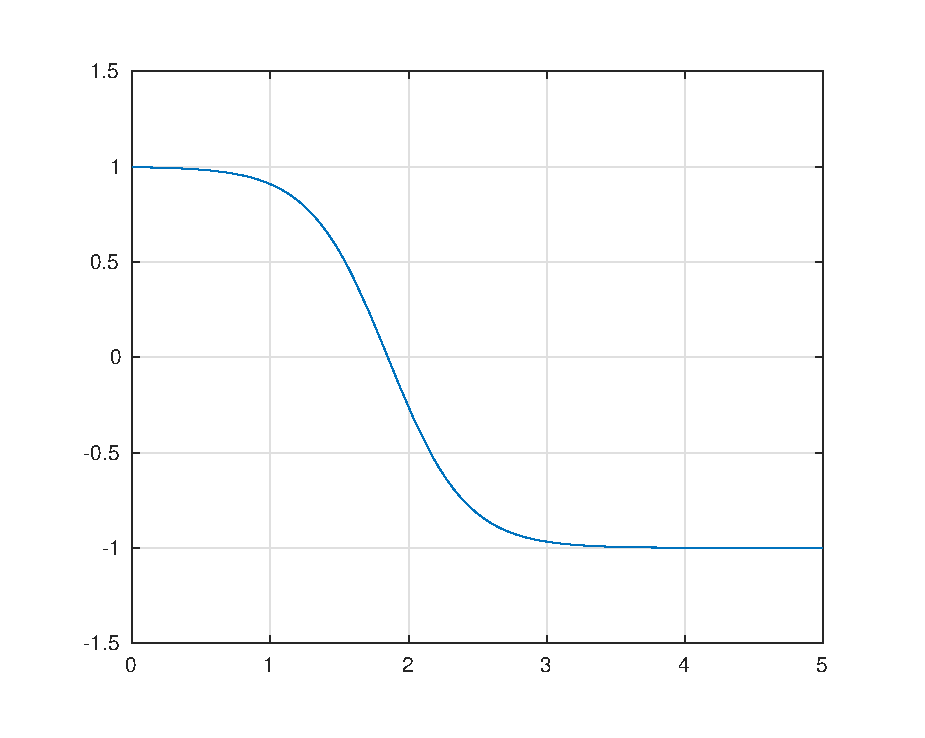
\includegraphics[width=0.5\textwidth]{figures/sig185.eps}
    \caption{Plot of the sigmoid function used to achieve the results in \Cref{tab:adjusting-SO-NO}.}
    \label{fig:sig185}
\end{figure}

\begin{table}[h]
\centering
\begin{tabular}{rlrrrr}
\hline
\textit{} & Category & \#Users & ANGA & ANIA & \#Imp. ND \\ \hline
\multirow{4}{*}{\textit{\begin{tabular}[c]{@{}r@{}}SO 2.0\\ NO 2.3\end{tabular}}} & +/+ & 6 & 139010 & 529 & 0 \\
 & +/- & 2 & 759945 & 4749 & 12 \\
 & -/+ & 24 & 4408 & 932 & 0 \\
 & -/- & 14 & 5110 & 3107 & 33 \\ \cline{2-6} 
 & Summary & 46 & 8973 & 1707 & 45 \\ \hline
\multirow{4}{*}{\textit{\begin{tabular}[c]{@{}r@{}}SO 2.3\\ NO 2.6\end{tabular}}} & +/+ & 5 & 13475 & 283 & 0 \\
 & +/- & 1 & 139525 & 5252 & 7 \\
 & -/+ & 35 & 3022 & 712 & 0 \\
 & -/- & 5 & 4071 & 2090 & 7 \\ \cline{2-6} 
 & Summary & 46 & 7240 & 914 & 14 \\ \hline
\multirow{4}{*}{\textit{\begin{tabular}[c]{@{}r@{}}SO 2.6\\ NO 2.9\end{tabular}}} & +/+ & 3 & 9372 & 251 & 0 \\
 & +/- & 1 & 139525 & 4335 & 5 \\
 & -/+ & 38 & 3041 & 596 & 0 \\
 & -/- & 4 & 3400 & 1499 & 6 \\ \cline{2-6} 
 & Summary & 46 & 6452 & 734 & 11 \\ \hline
\multirow{4}{*}{\textit{\begin{tabular}[c]{@{}r@{}}SO 3.0\\ NO 3.3\end{tabular}}} & +/+ & 3 & 9372 & 234 & 0 \\
 & +/- & 1 & 139525 & 4014 & 4 \\
 & -/+ & 38 & 2671 & 548 & 0 \\
 & -/- & 4 & 3396 & 1389 & 6 \\ \cline{2-6} 
 & Summary & 46 & 6146 & 676 & 10 \\ \hline
\multirow{4}{*}{\textit{\begin{tabular}[c]{@{}r@{}}SO 2.3\\ NO 3.3\end{tabular}}} & +/+ & 3 & 9372 & 249 & 0 \\
 & +/- & 1 & 139525 & 4747 & 7 \\
 & -/+ & 37 & 3064 & 556 & 0 \\
 & -/- & 5 & 3577 & 1646 & 7 \\ \cline{2-6} 
 & Summary & 46 & 6497 & 746 & 14 \\ \hline
\end{tabular}
\caption{CA results achieved by adjusting Single Occurrence (SO) and No Occurrences (NO) parameters. DTM parameters were $A = 1.85$, $B = 0.28$, $C = 1$ and $T_{\text{lockout}} = 90$.}
\label{tab:adjusting-SO-NO}
\end{table}

\subsection{Outlier removal}
\label{sec:analysis-CA-outliers}
In \Cref{sec:system-design-CA-ref}, we mentioned that we tested the CA system with and without outlier values in the reference.
When testing the system with these outliers removed, we observed a severe drop in both ANGA and ANIA ratings.
This essentially means that the system became more \textit{strict}, rapidly locking out both imposters and genuine users.
The reason for this lies in how our classifier (SMD) is scaled using standard deviation, which accounts for the dispersion of timing values.
The dispersion decreases when removing outliers, and a consequence is that the system expects keystroke features with less distance to the reference than before outlier removal.
Therefore, we had to make adjustments to the DTM's system level parameters to account for this change in expected user behavior.

The results in \Cref{tab:adjusting-SO-NO} were achieved \textit{without} outlier removal.
The parameters which gave an ANGA of 6146 and ANIA of 676 gave an ANGA of 1255 and ANIA of 218 when outliers were removed during reference construction.
We attempted to lower $T_{\text{lockout}}$ from 90 to 80 to make the system less strict, though this resulted in the ANIA rating increasing rapidly compared to the ANGA rating.
Specifically, it resulted in 4429 ANGA and 787 ANIA.
In other words, imposters gained too much of an advantage compared to the genuine user to justify this method for making the system more liberal.
%Lowering $T_{\text{lockout}}$ from 90 to 80 resulted in an ANGA of 4429 and ANIA of 787, which showed rapid growth of the ANIA rating compared to the ANGA rating's growth.

Lowering the DTM's "A" parameter to $1.3$ gave better results, which can be found in \Cref{tab:CA-outliers-removed-without-cutoff}.
These are comparable to the best result from \Cref{tab:adjusting-SO-NO}, being the 6146 ANGA and 676 ANIA.
Specifically the fourth row in \Cref{tab:CA-outliers-removed-without-cutoff} shows a result with 694 ANIA, only 18 actions more than the 676 ANIA without outlier removal.
Despite the small difference in ANIA ratings, the result \textit{with} outlier removal gave a significantly higher ANGA rating, as the genuine user could on average perform $8436-6146 = 2290$ more keypresses before being locked out.
With such positive results, we kept the outlier removal mechanism when combining the CA system with the PA system.
%The ANIA value of 676 \textit{without} outlier removal is comparable to the ANIA value of

\begin{table}[h]
\centering
\begin{subtable}[h]{0.45\textwidth}
\begin{tabular}{lrrr}
\hline
 $T_{\text{lockout}}$ & ANGA  & ANIA & \#Imp. ND  \\ \hline
 80                   & 1615  & 174  & 2          \\
 70                   & 3437  & 335  & 6          \\
 60                   & 5385  & 504  & 12         \\
 50                   & 8436  & 694  & 26         \\
 40                   & 10846 & 882  & 31         \\
 30                   & 12208 & 1103 & 50         \\
 20                   & 12981 & 1325 & 62         \\
 10                   & 13183 & 1503 & 69         
 \end{tabular}
 \caption{Without reference cutoff.}
 \label{tab:CA-outliers-removed-without-cutoff}
\end{subtable}
\hfill
\begin{subtable}[h]{0.45\textwidth}
\centering
\begin{tabular}{lrrr}
\hline
 $T_{\text{lockout}}$ & ANGA  & ANIA & \#Imp. ND \\ \hline
 80                   & 1569  & 159  & 2         \\
 70                   & 3283  & 299  & 5         \\
 60                   & 5297  & 450  & 10        \\
 50                   & 8362  & 625  & 21        \\
 40                   & 10622 & 798  & 25        \\
 30                   & 11871 & 1009 & 44        \\
 20                   & 12422 & 1180 & 52        \\
 10                   & 12727 & 1350 & 61       
\end{tabular}
\caption{With reference cutoff.}
\label{tab:CA-outliers-removed-with-cutoff}
\end{subtable}
\caption{CA results achieved with outlier removal using the following DTM parameters: $A= 1.3, B = 0.28 \text{ and } C=1$.}
\label{tab:CA-outliers-removed}
\end{table}

%\todo{Check all references to this chapter from System level chapter, and see if they need to be removed.}

\subsection{Reference cutoff}
\label{sec:analysis-cutoff}
When the individual CA and PA systems were implemented, a decision had to be made regarding the amount of keystroke data to be used in reference building.
As mentioned in \Cref{sec:system-design-dataset}, we use 35\% of the user's keystrokes recorded during data collection.
We tested the impact of limiting this amount to a maximum of 20000 keystrokes for users with exceptionally large datasets, so that the remaining training data could be used for testing instead.
Another motivating factor is that it leads to slightly less variance in reference quality between users.

The results in \Cref{tab:CA-outliers-removed} shows the impact of applying the reference cutoff.
We observed that both the ANGA and ANIA ratings as well as the number of undetected imposters generally were lowered as a consequence.
The difference was still minimal, and we concluded that it was reasonable to continue further analysis \textit{with} the reference cutoff.

\subsection{Personal and system level parameters}
\label{sec:CA-personal-parameters}
As our PA system has an element of \textit{personalization} in its lockout threshold, we faced the issue of personalizing the CA system as well before combining the systems.
The incentive to do so was that incorporating a personalized PA system into a CA system which only uses global parameters might be viewed as an unfair method for improving performance.
Therefore, we also built a version of our CA system which uses customized thresholds for rewards/penalties for each user.
\Cref{sec:CA-trust-and-decision} describes how the thresholds are calculated by using mean scores and tolerance levels.
The SO and NO parameters were then locked at 5, to ensure that users were punished for typing rarely or never before seen n-graphs, even with these customized thresholds.

Adjusting the tolerance level led to the results presented in \Cref{tab:CA-persRwrdThresh}, where using a tolerance level of 0.5 led to the most reasonable performance.
It was achieved with $T_{\text{lockout}}=50$, and can be compared to the result in \Cref{tab:CA-outliers-removed-with-cutoff} where also $T_{\text{lockout}} = 50$.
Whereas the ANIA dropped by an insignificant amount, the ANGA dropped from 8362 to 8087.
Though this was a negative change, the number of undetected imposters also dropped from 21 to 18, which slightly weighs up for the loss of ANGA rating.
Overall, these settings gave a satisfying performance and were used as the base when incorporating the PA system.

\begin{table}[h]
\centering
\begin{tabular}{lrrr}
\hline
Toler. & ANGA  & ANIA & \#Imp. ND  \\ \hline
0   & 268   & 69  & 0  \\
0.1 & 770   & 93  & 0  \\
0.2 & 2107  & 143 & 3  \\
0.3 & 3951  & 218 & 3  \\
0.4 & 5671  & 381 & 5  \\
0.5 & 8087  & 623 & 18 \\
0.6 & 10461 & 986 & 36
\end{tabular}
\caption{CA results achieved with personal thresholds for reward/penalty. DTM parameters: \\$A=\text{ personal}, B = 0.28, C=1\text{, and } T_{\text{lockout}} = 50$.}
\label{tab:CA-persRwrdThresh}
\end{table}

\section{PA system}
\label{sec:analysis-PA}
\subsection{Reference cutoff}
The PA system's performance was tested with and without the reference cutoff, similarly to the CA tests discussed in \Cref{sec:analysis-cutoff}.
\Cref{tab:PA-cutoff} shows the cutoff's impact on performance. 
As in the case of the CA system, the impact is negligible.
Adjusting the tolerance level allowed us to balance the relation between FNMR and FMR, as mentioned in \Cref{sec:system-design-PA-decision}.
In other words, this parameter decided the system's strictness.
%The goal was to find a reasonable balance which had a high chance of detecting imposters 
%thereby controlling the tradeoff of catching imposters more quickly and locking out the genuine user more often.

%When combining the CA and PA systems, the same sets of keystrokes had to be used to build their references, as well as their test sets.
%When combining the CA and PA systems, the datasets had to be separated into references, validation sets and test sets in an identical manner.
The users' datasets had to be separated into references, validation sets and tests sets in an identical manner for the CA and PA systems.
This was needed due to the combined system using the exact same keystroke data for both the CA and PA subsystems during testing.
If the reference cutoff was used in only one of the subsystems, the test sets would contain different keystrokes, as the cutoff causes data from the reference portion of the dataset to be moved into the test portion.
The advantages given by the cutoff described in \Cref{sec:analysis-cutoff} also hold for the PA system.
Seeing as the impact of the cutoff was small for both systems, the cutoff was used in further analysis. This included testing of the combined system.

\begin{table}[h]
\centering
\begin{subtable}[h]{0.45\textwidth}
\begin{tabular}{lrrr}
\hline
Toler. & FNMR & FMR & \#Imp. ND  \\ \hline
0.02 & 47.51 & 4.68  & 2   \\
0.06 & 37.75 & 5.93  & 4   \\
0.10  & 30.25 & 7.47  & 4   \\
0.14 & 22.97 & 9.23  & 7   \\
0.18 & 17.77 & 11.48 & 9   \\
0.22 & 13.40 & 14.07 & 13  \\
0.26 & 9.44  & 17.11 & 17  \\
0.30 & 6.91  & 20.52 & 22  \\
0.35 & 4.70  & 25.37 & 37  \\
0.40 & 2.85  & 30.80 & 54  \\
0.45 & 1.80  & 36.67 & 87  \\
0.50 & 1.29  & 42.61 & 121
 \end{tabular}
 \caption{Without reference cutoff.}
 \label{tab:PA-without-cutoff}
\end{subtable}
\hfill
\begin{subtable}[h]{0.45\textwidth}
\centering
\begin{tabular}{lrrr}
\hline
Toler. & FNMR  & FMR & \#Imp. ND \\ \hline
0.02 & 48.08 & 4.68  & 2   \\
0.06 & 38.54 & 5.94  & 4   \\
0.10 & 30.04 & 7.50  & 4   \\
0.14 & 22.59 & 9.37  & 7   \\
0.18 & 17.36 & 11.70 & 9   \\
0.22 & 12.89 & 14.28 & 12  \\
0.26 & 9.29  & 17.42 & 18  \\
0.30 & 6.44  & 20.91 & 21  \\
0.35 & 3.85  & 25.88 & 36  \\
0.40 & 2.26  & 31.47 & 53  \\
0.45 & 1.51  & 37.45 & 88  \\
0.50 & 1.13  & 43.55 & 126
\end{tabular}
\caption{With reference cutoff.}
\label{tab:PA-with-cutoff}
\end{subtable}
\caption{Excerpt of PA results showing the performance impact of using a reference cutoff. A block size of 500 keystrokes was used. A complete version on this table is found in \Cref{sec:app-PA-reference-cutoff}.}
\label{tab:PA-cutoff}
\end{table}

\subsection{R- and A-distance weights}
Pinto et al. \cite{Pinto2014} studied how adjusting the weights of the R-and A-distances when combining them affected detection performance.
They found that 20\%-80\% weights for R- and A-distances was the best configuration for increasing the gap between average genuine and imposter scores while still considering the R-measure.
We tested our PA system using the same configuration to see how it affected its performance.
The result is illustrated as Detection error tradeoff (DET) curves in \Cref{fig:RAweights}.
The curves show that summing the R-and A-distances with equal weights outperforms the 80-20 weighting scheme for our PA system, as all FNMRs give lower tradeoffs for FMR with the equal weights scheme.

While we did not analyze the underlying reasons, it is worth pointing out that Pinto et al. used five different timing features where our system only uses three.
We also used a smaller block size of 500 keystrokes compared to their 750 keystrokes, and as mentioned in \Cref{sec:system-design-PA-comparison}, their dataset was limited.
All of these factors could play a role in why we had less success with their weighting scheme.
As we were not looking for the optimal PA solution, we did not test to see if other weights were better. 
Equal weights were chosen for further analysis due to the superior performance.

\begin{figure}[ht]
    \centering
    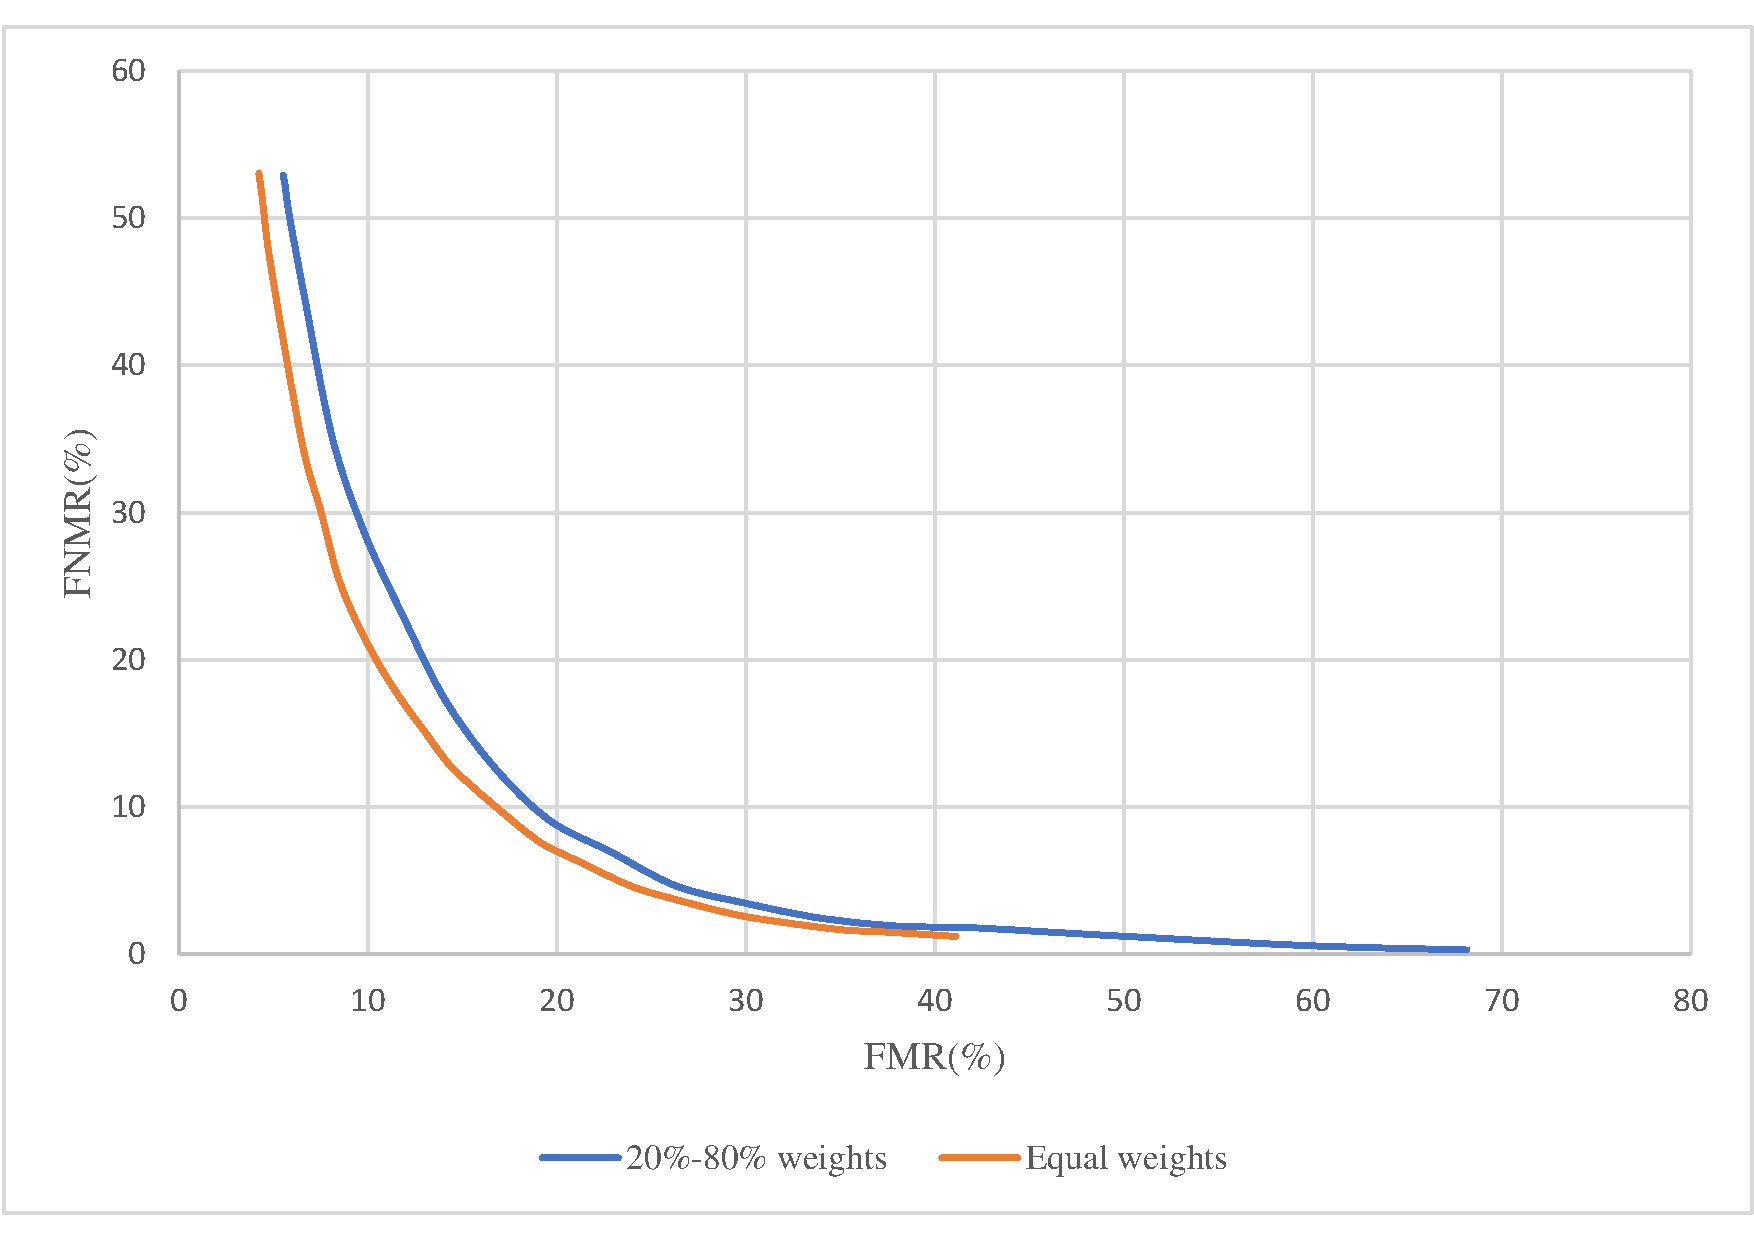
\includegraphics[width=1\textwidth]{figures/weights.pdf}
    \caption{Detection error tradeoff curves showing the detection performance of weighing R- and A-distances by 20-80\% respectively as well as using equal weights. }
    \label{fig:RAweights}
\end{figure}


\subsection{Block size}
\label{sec:analysis-PA-block-size}
Different block sizes were tested for the PA system.
These were 500, 250 and 100 keystrokes.
As a dissimilarity score is produced per block, the system has more information to base every dissimilarity score on when the block size is large.
This generally leads to more accurate decisions per block, and is reflected in the DET curves in \Cref{fig:block-lengths-ROC}.
There is a clear difference in detection accuracy between the block lengths that were tested, with 500 outperforming both of the other block sizes, and size 100 achieving the worst performance in terms of detection accuracy.

\begin{figure}[h]
    \centering
    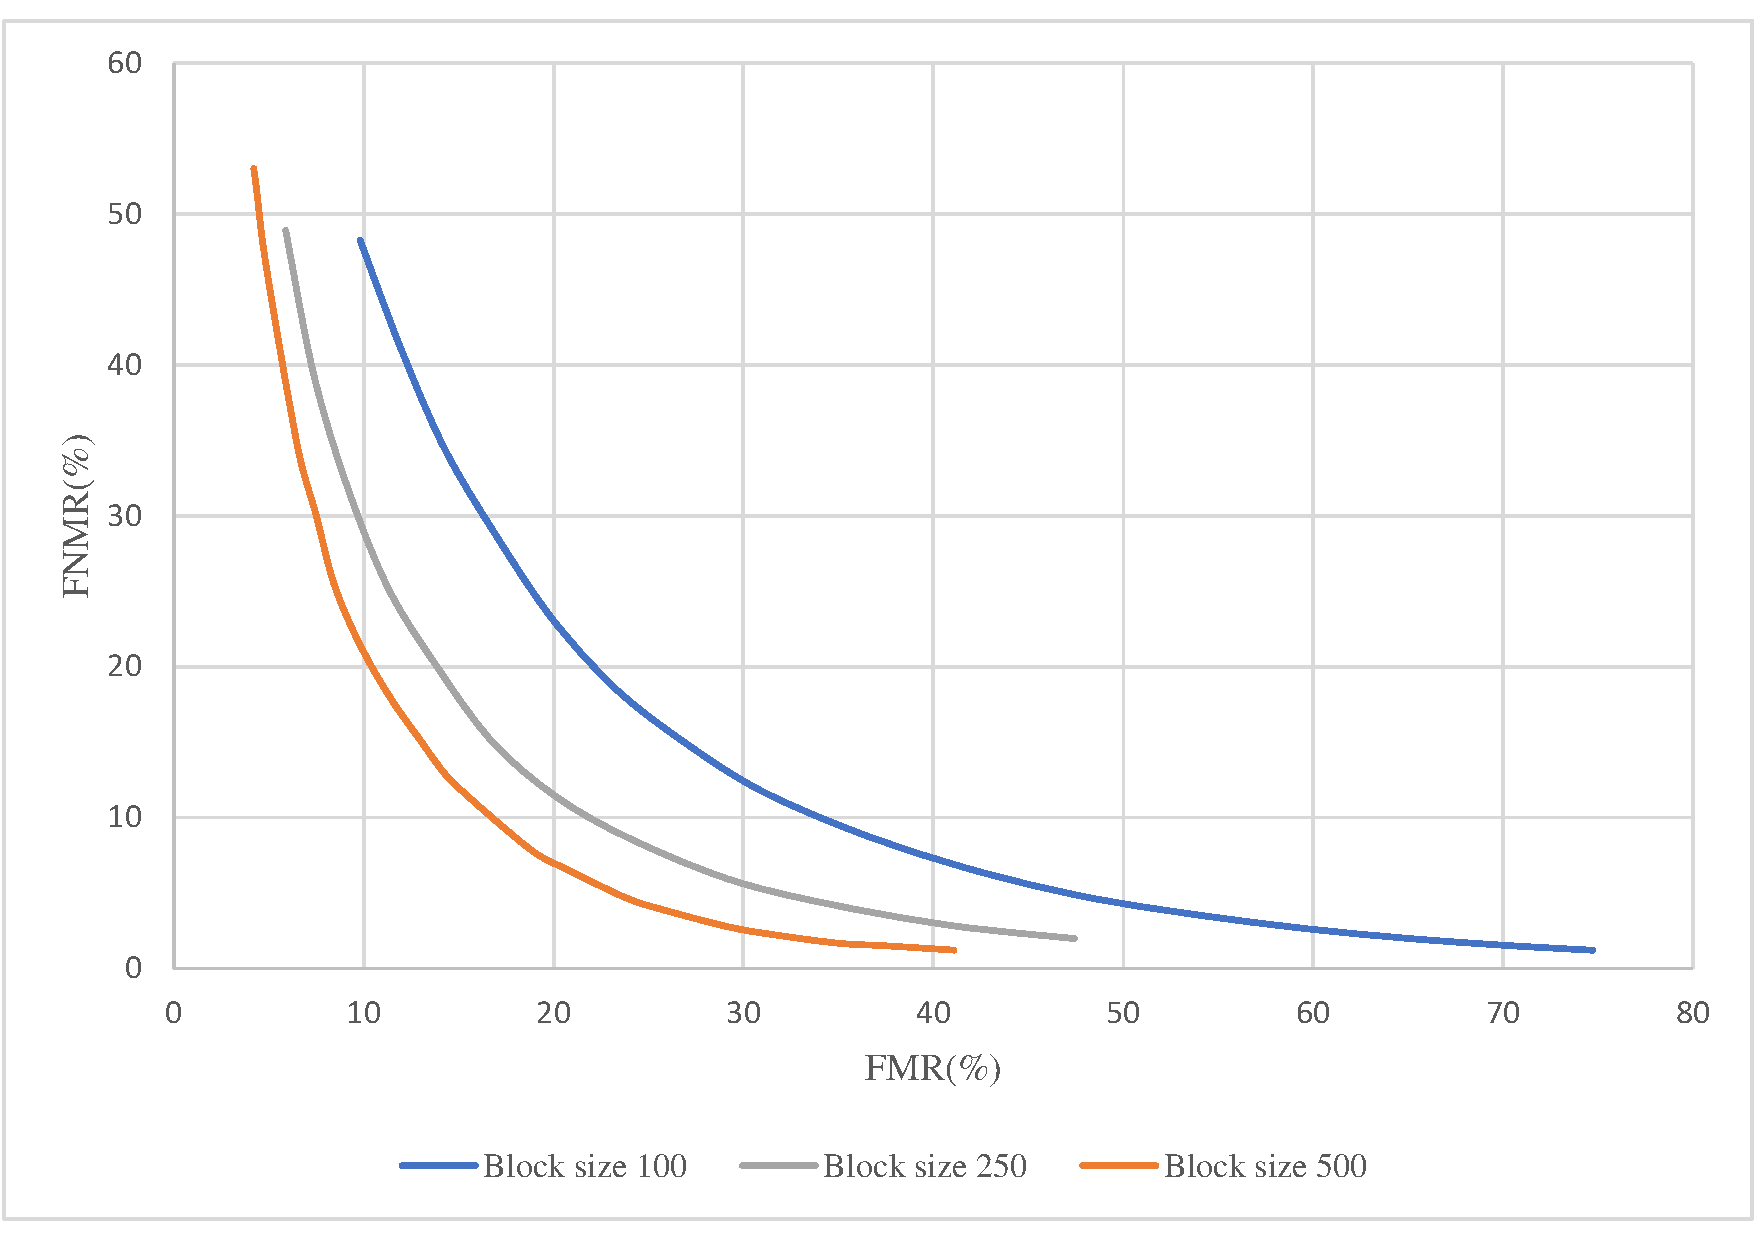
\includegraphics[width=1\textwidth]{figures/PA-BLs-ROC.pdf}
    \caption{DET curves showing the performance for different block sizes.}
    \label{fig:block-lengths-ROC}
\end{figure}

This does not necessarily imply that using a block size of 500 gives a \textit{better} PA system.
When the PA system waits for 500 keystrokes to be collected before processing probes, the imposter has a large window of access to the computer before they are locked out.
An example of an unfortunate scenario could be an imposter taking control over an unattended computer after the genuine user had either logged in or been successfully authenticated by the PA system without pressing any keys thereafter.
In both of these cases, the imposter would have free reign over the computer until they had typed 500 keystrokes, or until the genuine user returned to the workstation.

At first glance, this may seem like the worst-case scenario.
However, the imposter could also take control over the computer in the middle of a block, for example after 300 genuine keystrokes.
Ideally, they would be detected and locked out when the block was filled up, i.e. after only $500-300 = 200$ imposter keystrokes.
However, their window of opportunity could also become larger than 500.
The reason for this is that the genuine keystrokes making up the first 300 keystrokes of the block may outweigh the 200 imposter keystrokes, causing the probe to be accepted as \textit{genuine}, i.e. a match.
The PA system would then continue collecting keystrokes for the next block without locking the imposter out.
Their effective window of opportunity would then be $200+500 = 700$, giving them increased time to perform potentially harmful actions.

Situations like these highlight fundamental issues with PA systems and why such large block sizes can be problematic.
There is a tradeoff between higher detection performance and lower block sizes, which is why we tested the system with several block sizes.
All of these block sizes could then be used for testing the combined system later on.

\begin{table}[h]
\centering
\begin{subtable}[h]{0.45\textwidth}
\begin{tabular}{lrrr}
\hline
Toler. & ANGA  & ANIA & \#Imp. ND  \\ \hline
0.35 & 12989 & 675 & 36 \\
0.33 & 10670 & 656 & 31 \\
0.3  & 7760  & 632 & 21 \\
0.26 & 5383  & 605 & 18 \\
0.22 & 3880  & 583 & 12 \\
0.18 & 2880  & 566 & 9  \\
0.14 & 2213  & 552 & 7  \\
0.1  & 1664  & 541 & 4  \\
0.06 & 1298  & 532 & 4
 \end{tabular}
 \caption{Block size 500.}
 \label{tab:PA-block-size-500}
\end{subtable}
\hfill
\begin{subtable}[h]{0.45\textwidth}
\centering
\begin{tabular}{lrrr}
\hline
Toler. & ANGA  & ANIA & \#Imp. ND \\ \hline
0.5  & 12634 & 476 & 52 \\
0.45 & 8957  & 426 & 31 \\
0.43 & 7845	 & 409 & 27 \\
0.4  & 6124  & 386 & 19 \\
0.35 & 4302  & 354 & 16 \\
0.3  & 2920  & 329 & 11 \\
0.26 & 2198  & 313 & 8  \\
0.22 & 1665  & 300 & 6  \\
0.18 & 1252  & 290 & 2  
\end{tabular}
\caption{Block size 250.}
\label{tab:PA-block-size-250}
\end{subtable}

\begin{subtable}[h]{0.45\textwidth}
\centering
\begin{tabular}{lrrr}
\hline
Toler. & ANGA  & ANIA & \#Imp. ND \\ \hline
0.7  & 8288 & 395 & 98 \\
0.65 & 6531 & 335 & 66 \\
0.6  & 5028 & 286 & 38 \\
0.55 & 3779 & 247 & 30 \\
0.45 & 2112 & 192 & 12 \\
0.35 & 1136 & 157 & 3  \\
0.26 & 672  & 137 & 1  \\
0.18 & 433  & 125 & 0  \\
0.1  & 289  & 117 & 0  
\end{tabular}
\caption{Block size 100.}
\label{tab:PA-block-size-100}
\end{subtable}

\caption{Excerpt of PA results achieved with different block sizes and tolerance levels.}
\label{tab:PA-block-sizes}
\end{table}

The ANGA and ANIA rates of the PA system are calculated based on FNMR and FMR rates and are presented in \Cref{tab:PA-block-sizes}, where the performance of the block sizes can be further compared.
An immediate observation is that small blocks sizes give lower ANIA rates than larger block sizes when similar ANGA rates are compared.
For example, when comparing results with approximately 2000 ANGA, the respective ANIA rates for block sizes 500, 250 and 100 are around 552, 313 and 192.
If we were to judge the performance solely based on ANGA and ANIA rates, it would seem that small block sizes are better.
However, the smaller block sizes tend to have significantly more undetected imposters.
Also, with higher ANGA rates, the smaller block sizes cause the system to often need more than one block to catch imposters.
While this is not necessarily a large issue in a stand-alone PA system with such small block sizes, problems can arise when combined with the CA system.
If the PA system can influence the trust level to be \textit{increased}, then the blocks that produce a false match before the imposter is detected will boost the trust level.
This can negate the CA system's own progress in detecting the imposter.
For instance, if the imposter's current trust level is 60, and $T_{\text{lockout}}=50$, a falsely matched block could increase the current trust level back to for example 90.
This would give the imposter a larger window of opportunity than if the PA system was not involved in the first place, as the CA system probably would have brought the trust level below $T_{\text{lockout}}$ a few moments later.
Smaller block sizes are therefore not necessarily the better option for the combined system.


\section{Decision level fusion}
\label{sec:analysis-decision-lvl}
This section presents results achieved by combining continuous and periodic authentication at the decision level.
The fusion scheme is based on the allowed range of trust $T_\text{range}$ as described in \Cref{sec:system-design-combined-score}.
As the CA configuration chosen for the combined system had $T_{\text{lockout}} = 50$, the allowed range of trust was $T_{\text{range}} = 100-50 = 50$.
When testing the decision level fusion, the binary decision of the PA subsystem would therefore increase or decrease the trust level by a specific amount between 0-50.
%Results from the decision level fusion are shown in \Cref{sec:analysis-decision-lvl}, while score level fusion results can be found in \Cref{sec:analysis-score-lvl}.
%The section is concluded with a discussion in \Cref{sec:analysis-discussion}.




%\subsection{}
%As described in \Cref{sec:system-design-combined-decision}, the decision level fusion scheme has the PA subsystem processing a probe block and sending a Match or Non-Match result to the CA system's DTM.
%The DTM then adjusts the current trust level according to the received result, by lowering or increasing it by specific amounts.

In order to control how much to increase or decrease the trust level, two parameters were used.
They were \textit{'UP'} and \textit{'DOWN'}, 
each representing how large a portion of $T_{\text{range}}$ to increase or decrease the current trust level by, respectively.
For instance, with $\textit{UP}=0.3$ and $\textit{DOWN}=0.6$, probe blocks producing a match would increase the trust level by $0.3 \times 50 = 15$.
Probes producing a non-match would decrease the trust level by $0.6 \times 50 = 30$.
Such a configuration would punish imposters more than it would reward the genuine user.
%Therefore, it would lock out imposters quicker, and cause reduced damage if they were falsely believed to be the genuine user.

The \textit{UP} and \textit{DOWN} values were set as system level parameters, i.e. they were the same for all users per test.
Optimizing these values for each user using genetic algorithms or other optimization techniques is another option.
Such algorithms are however computationally expensive and time consuming, and were not used for this project.

An example of a setting that we tested was $\textit{UP}=1$ and $\textit{DOWN}=0.6$.
\Cref{fig:decision-lvl-genuine-250BL} shows an excerpt of testing this setting with User 1 as a genuine user, meaning that their test set was used against their own reference.
In the beginning, the user seemed to be typing in an unusual manner compared to their reference causing the CA subsystem to rapidly decrease the trust level.
After 108 keystrokes, the trust level went below $T_{\text{lockout}}$, marking the undesired event of locking out the genuine user.
The block size was 250 in this case, and since the CA subsystem locked out the user before the block was filled up, the PA subsystem did not get a chance to prevent the lockout.

\begin{figure}[htbp]
\centering
\begin{subfigure}[b]{0.8\textwidth}
   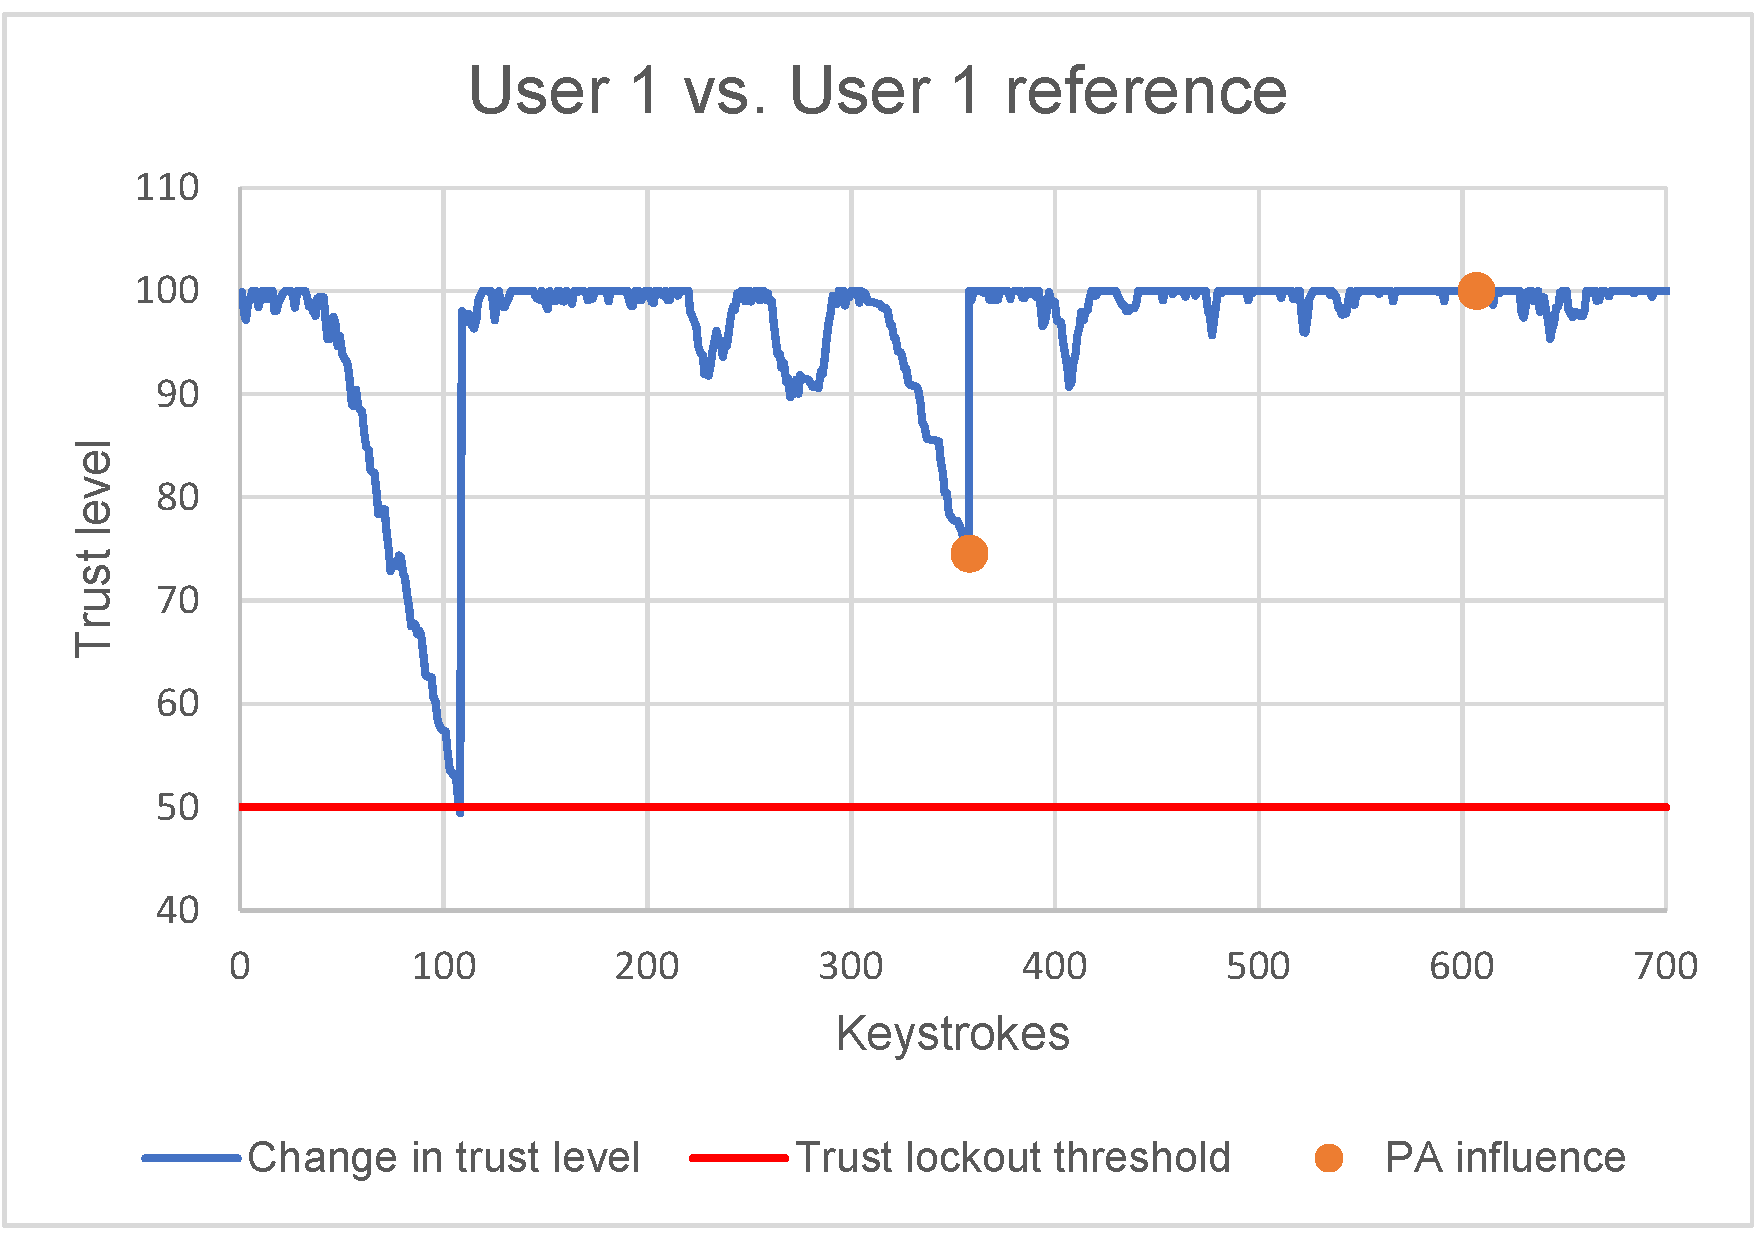
\includegraphics[width=1\linewidth]{figures/decision-lvl-genuine-250BL.pdf}
   \caption{User 1 as genuine user.}
   \label{fig:decision-lvl-genuine-250BL} 
\end{subfigure}

\begin{subfigure}[b]{0.8\textwidth}
   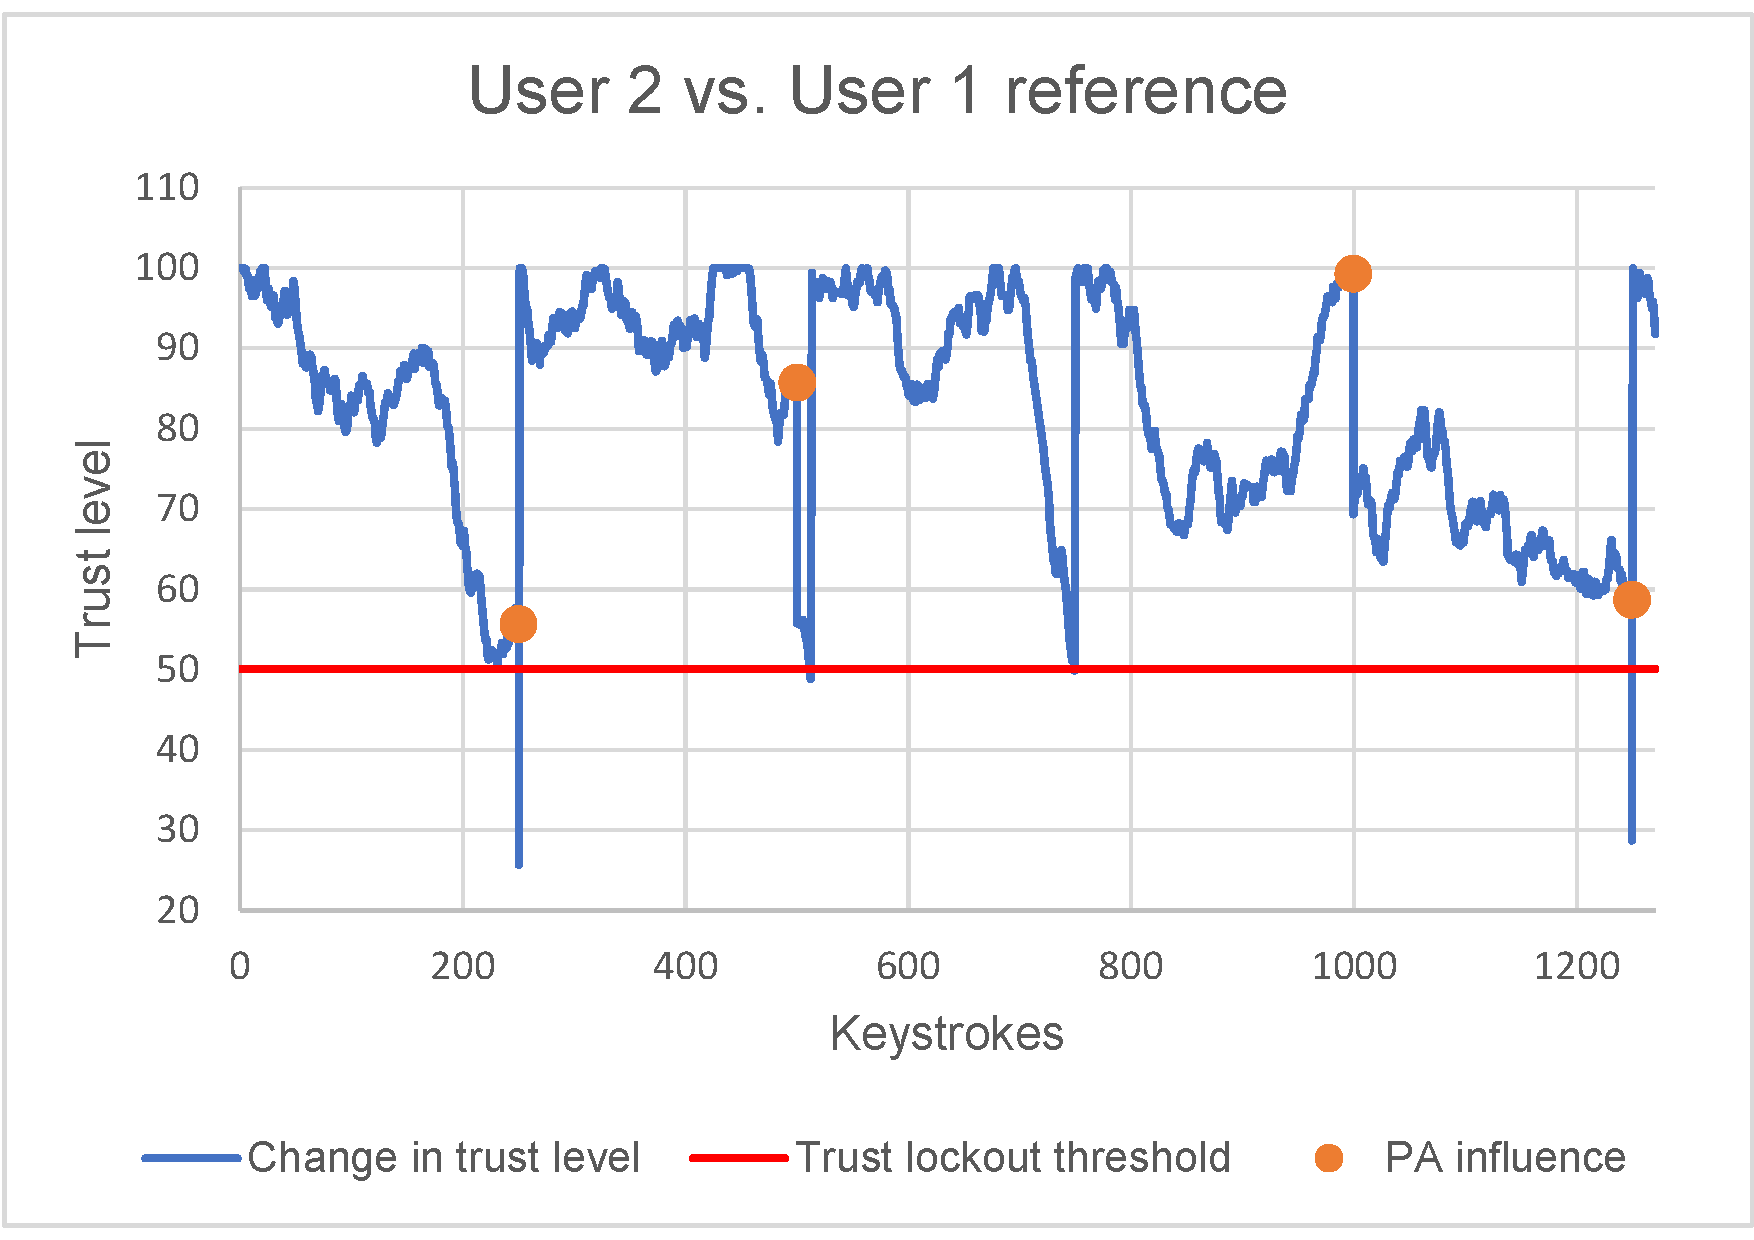
\includegraphics[width=1\linewidth]{figures/decision-lvl-user2-vs-user1-250BL.pdf}
   \caption{User 2 as imposter vs User 1's reference.}
   \label{fig:decision-lvl-user2-vs-user1-BL250}
\end{subfigure}

\caption{Examples of decision level fusion with $\text{block size} = 250$. $\textit{UP} = 1, \textit{DOWN} = 0.6$.}
\label{fig:decision-lvl-user1-example}
\end{figure}

The trust level was brought back up to 100 after the lockout, which simulated the user logging back in and continuing typing.
The PA subsystem started collecting keystroke data for a new block from that point onward.
After keystroke number 300, the trust level started sinking again, down to 75 at keystroke number 358.
At that point, a block of 250 keystrokes had been filled up since the lockout at keystroke number 108.
This triggered the PA system to process the block probe, which resulted in a match.
Here we can observe the advantage of combining the systems, as the PA match caused the trust level to be increased by $1 \times 50 = 50$, capped at the maximum value of 100.
Such positive adjustments have the potential to give the genuine more time before potentially being wrongfully locked out.
In this specific example, we can see that another block was filled up, processed and matched after the following 250 keystrokes, however the trust level was at that point already at 100.

\Cref{fig:decision-lvl-user2-vs-user1-BL250} shows a portion of a test run where an imposter was locked out four times over the course of around 1250 keystrokes.
At keystroke number 231, the trust level dipped to 50.2 before increasing slightly again, barely keeping the imposter logged in.
However, at keystroke number 250, the PA subsystem kicked in and reduced the trust level by $0.6 \times 50 = 30$, bringing it far below $T_{\text{lockout}}$.
As this meant that the imposter was locked out, the trust level was then brought back to 100, and the test run continued.

Keystroke number 500 shows another example of the cooperation between the two subsystems.
The PA subsystem brought the trust level down by 30, which was not quite enough to bring it below the threshold.
The CA subsystem was however able lock the user out a few keystrokes later due to the assistance it received just before.
Later on, the CA subsystem locked the imposter out at keystroke number 749, just one keystroke before the PA subsystem would have kicked in.
After that, the CA subsystem was unable to cause another lockout on its own.
However, at keystroke number 999, the PA subsystem brought the trust level down to 70, and later on brought it below the threshold at keystroke 1249.
Especially the last two PA influences show how using the statistical information available in block probes can be beneficial to utilize in a combined CA/PA system.


\subsection{Results}
\label{sec:analysis-decision-lvl-results}
Before looking at how the incorporation of the PA system had an influence on the original CA system's performance, we will discuss some observations regarding the impact of the decision level fusion's parameters.
The first observation to mention is that adjusting the \textit{DOWN} parameter generally had a larger impact on detection performance than the \textit{UP} parameter.
An example of this can be seen in \Cref{tab:UD-difference-1.001,tab:UD-difference-0.4}, as the performance difference between them was negligible even with a considerable difference in \textit{UP} values.
However, adjusting the \textit{DOWN} parameter from 0 to 1.001 caused a difference of over 2500 ANGA and over 340 ANIA.
The reason for testing $\textit{DOWN}=\text{1.001}$ was the same as explained in \Cref{sec:system-design-combined-score}; it allowed the PA subsystem's influence to cause a direct lockout even when the current trust level was at its maximum.
As seen in the tables, the extra 0.001 in \textit{DOWN} value showed its effect by causing a drop in both ANGA and ANIA. 
However, the ANGA showed a drop of $6366-6018 = 348$ in \Cref{tab:UD-difference-0.4}, while the ANIA only dropped by $306-298 = 8$.
%In the same table we can see similar drops in ANGA where the corresponding ANIA drop is around 50.
%What this means is that the benefit of being able to lock out imposters who are currently at trust level 100 is small compared tcatching imposters 8 keystrokes earlier on average has a large negative consequence
This indicates that letting the PA subsystem lock out users who are currently at trust level 100 has large consequences for genuine users compared to the benefit of locking out imposters faster.
This makes sense, as a user at trust level 100 is more likely to be the genuine user than an imposter.
When these genuine users are wrongfully brought from trust level 100 to below $T_{\text{lockout}}$, the CA subsystem is given no chance to correct the PA subsystem's mistake.
Since imposters spend more time below trust level 100, reducing their trust level by $1\times T_{\text{range}}$ will often bring them far below $T_{\text{lockout}}$ which could be considered an "overkill".
Therefore, the extra 0.001 punishment is less likely to make a difference for them than for genuine users.
This ties into our \textit{research sub-question 2}, as it seems that having the PA subsystem adjust the trust level is generally better than guaranteeing that a non-match results in an instant lockout.
In spite of this, we continued testing $\textit{DOWN} = \text{1.001}$ to see if similar behavior was shown for other settings as well.

The reason for testing $\textit{UP} = \text{1.001}$ instead of 1 is simply that we originally tested the system using equal values for \textit{UP} and \textit{DOWN}, and $\textit{DOWN} = \text{1.001}$ was needed for the reason mentioned above.
The extra 0.001 for the \textit{UP} parameter makes no difference in practice, and was only used for convenience.
What does however make a difference for the \textit{UP} parameter is giving it a low value, usually below 0.4.
At such low values, the tests showed an exception to the general behavior being that adjustment of \textit{UP} makes little to no difference.
This can be seen in \Cref{tab:UD-difference-0.2}, where $\textit{UP} = \textit{0.2}$.
When comparing these results to the other two tables, we can see that it gave lower ANGA ratings for similar ANIA ratings.
In other words, using such a low \textit{UP} gave a worse performance across the board.

A likely explanation is that some genuine users have benefited largely by being ‘saved’ by the PA system at certain times, when their trust level was low.
With smaller \textit{UP} values, the PA subsystem had less power in preventing the CA subsystem from wrongfully locking them out, and so the small boost in trust level may not have been enough to keep them logged in for much longer.
Therefore, most of the following results presented in this section were achieved using a high \textit{UP} value.
%While we have tested various \textit{UP/DOWN} combinations, most of the results in this section will be summarized and presented with equal values for the two parameters due to the low impact of the UP value.
%In other words, they will represent the performance of equally rewarding genuine users and punishing imposters.
%We will also show certain exceptions, i.e. where adjusting the \textit{UP} parameter caused interesting and positive results. 


\begin{table}[ht]
\centering
\begin{subtable}[h]{0.45\textwidth}
\begin{tabular}{lrrr}
\hline
\textit{DOWN} & ANGA  & ANIA & \#Imp. ND \\ \hline
%0     & 8944 & 706 & 25(1.2\%) \\
%0.2   & 8602 & 630 & 20(1\%)   \\
%0.4   & 8025 & 569 & 16(0.8\%) \\
%0.6   & 7380 & 499 & 12(0.6\%) \\
%0.8   & 7062 & 432 & 12(0.6\%) \\
%1     & 5604 & 284 & 3(0.1\%)  \\
%1.001 & 5239 & 273 & 2(0.1\%) THIS IS BL250 WITH 1.001 UP.
0     & 8547 & 644 & 19(0.9\%) \\
0.2   & 8545 & 605 & 18(0.9\%) \\
0.4   & 8263 & 564 & 15(0.7\%) \\
0.6   & 8089 & 508 & 11(0.5\%) \\
0.8   & 7676 & 445 & 8(0.4\%)  \\
1     & 6278 & 307 & 3(0.1\%)  \\
1.001 & 6019 & 299 & 3(0.1\%)  
\end{tabular}
 \caption{\text{$\textit{UP}=1.001$}}
 \label{tab:UD-difference-1.001}
\end{subtable}
\hfill
\begin{subtable}[h]{0.45\textwidth}
\centering
\begin{tabular}{lrrr}
\hline
\textit{DOWN} & ANGA  & ANIA & \#Imp. ND  \\ \hline
%0     & 8936 & 690 & 25(1.2\%) \\
%0.2   & 8594 & 620 & 20(1\%)   \\
%0.4   & 8017 & 557 & 16(0.8\%) \\
%0.6   & 7352 & 493 & 12(0.6\%) \\
%0.8   & 7068 & 426 & 12(0.6\%) \\
%1     & 5607 & 282 & 3(0.1\%)  \\
%1.001 & 5223 & 270 & 2(0.1\%) THIS IS BL250 WITH 0.4 UP
0     & 8543 & 642 & 19(0.9\%) \\
0.2   & 8541 & 603 & 18(0.9\%) \\
0.4   & 8261 & 563 & 15(0.7\%) \\
0.6   & 8088 & 507 & 11(0.5\%) \\
0.8   & 7676 & 444 & 8(0.4\%)  \\
1     & 6366 & 306 & 3(0.1\%)  \\
1.001 & 6018 & 298 & 3(0.1\%)  
 \end{tabular}
\caption{$\textit{UP} = 0.4$}
\label{tab:UD-difference-0.4}
\end{subtable}
\begin{subtable}[h]{0.45\textwidth}
\centering
\begin{tabular}{lrrr}
\hline
\textit{DOWN} & ANGA  & ANIA & \#Imp. ND  \\ \hline
0     & 8134 & 638 & 19(0.9\%) \\
0.2   & 8132 & 599 & 18(0.9\%) \\
0.4   & 7850 & 558 & 15(0.7\%) \\
0.6   & 7676 & 503 & 11(0.5\%) \\
0.8   & 7264 & 441 & 8(0.4\%)  \\
1     & 5869 & 304 & 3(0.1\%)  \\
1.001 & 5612 & 296 & 3(0.1\%)  
 \end{tabular}
\caption{$\textit{UP} = 0.2$}
\label{tab:UD-difference-0.2}
\end{subtable}

\caption{Differences in performance when adjusting \textit{DOWN} parameter for different \textit{UP} values. Block size was 500 and PA tolerance was 0.33.}
\label{tab:UD-difference}
\end{table}

In this analysis, we will mainly focus on two types of performance improvement introduced by the combination, both regarding ANGA and ANIA ratings.
Recall that the specific settings used for the CA subsystem resulted in 8087 ANGA and 623 ANIA.
Our focus areas are then as follows:

\begin{description}
    \item [ANGA improvements:] For settings giving around 623 ANIA, we are interested in ANGA ratings above 8087.
    \item [ANIA improvements:] Where the ANGA ratings are around 8087, we are looking for ANIA ratings below 623.
\end{description}
Some other results of interest will also be discussed, such as how far up the combination was able to boost the ANGA beyond the original system while accepting the compromise of a higher ANIA.

\subsubsection{Block size 500}
After having described the general effects of the \textit{UP} and \textit{DOWN} parameters, we can discuss how the original CA system's performance was affected by incorporating the PA system, which was the main goal of the analysis phase.
The first block size tested was 500 keystrokes.
From the PA results in \Cref{tab:PA-block-size-500}, we chose to use a tolerance level of 0.33, as it gave an ANGA of 10670 and ANIA of 656.
Having such a high ANGA while still having an ANIA comparable to the CA system's ANIA of 623 seemed beneficial for the combined system, and was the reason for choosing this PA setting.
The underlying FNMR and FMR rates which were used for calculating the ANGA and ANIA were 4.69\% and 23.8\%, respectively.
%The original CA system's performance is presented with more detail in \Cref{tab:CA-detailed-performance}.

Looking back at \Cref{tab:UD-difference-1.001}, we can see that the mentioned PA configuration was indeed able to positively affect the CA system's performance.
With $\textit{DOWN} = \text{0.2}$, the results were a higher ANGA for a slightly lower ANIA.
Specifically, the genuine users were able to type $8545-8087 = 458$ more keystrokes on average before being locked out, which is an increase of 5.66\%.
The ANIA was impacted more heavily, as seen where $\text{DOWN} = \text{0.6}$.
With an almost identical ANGA to that of the original CA system, the ANIA was lowered by $\text{623}-\text{508} = \text{115}$ which is an improvement of 18.46\%.
This means that imposters were caught significantly quicker on average with the combined system, supporting our main research question.
Also, the number of imposters that were never detected was reduced from 18 to 11.
This setting gave the best result for decreasing ANIA that we were able to find in this project.

Lastly, we can point out that for this block size, the ANGA saturated around 8545.
Increasing it any further beyond that point only resulted in a worse ANIA.
However, by sacrificing $\text{8087} - \text{6278} = \text{1809}$ ANGA, the ANIA dropped by 50.72\% down to 307, as seen where $\textit{DOWN} = \text{1}$.
With that setting, only 3 out of 2070 imposters were undetected.
%The general observed behavior of the decision level fusion is that increasing the \textit{U/D} values causes a decrease of both ANGA and ANIA.
%IS THIS DESCRIBED EARLIER?


%As \Cref{tab:UD-difference-BL500} shows an excerpt of the results achieved for the mentioned configuration, we refer to it for the discussion of this specific setting.
%Our first observation was that the ANGA rating peaked when \textit{UP and DOWN} (\textit{U/D}) was 0.3.
%The general observed behavior of the decision level fusion is that increasing the \textit{U/D} values causes a decrease of both ANGA and ANIA.
%However, these specific results show that only the ANIA increases when \textit{U/D} goes below 0.3, while the ANGA decreases.
%Strictly speaking, this is the opposite of what is wanted from a system like ours, as the optimal development would be an increasing ANGA coupled with a decreasing ANIA.
%A likely explanation is that one or more genuine users have benefited largely by being ‘saved’ by the PA system at certain times. 
%The less impact the \textit{UP} parameter is given, the less impact the boost of trust level has, and so the boost may not have been enough to keep them logged in.
%This is however a special behavior that was not seen in other block sizes, and is probably specific to our dataset.


%\begin{table}[ht]
%\centering
%\begin{tabular}{lrrr}
%\hline
%\textit{U/D} & ANGA  & ANIA & \#Imp. ND \\ \hline
%0.1   & 8087 & 608 & 17(0.8\%) \\
%0.2   & 8132 & 599 & 18(0.9\%) \\
%0.3   & 8332 & 580 & 15(0.7\%) \\
%0.4   & 8261 & 563 & 15(0.7\%) \\
%0.5   & 8130 & 542 & 14(0.7\%) \\
%0.6   & 8086 & 508 & 11(0.5\%) \\
%0.7   & 7819 & 475 & 8(0.4\%)  \\
%0.8   & 7676 & 445 & 8(0.4\%)  \\
%0.9   & 7361 & 388 & 5(0.2\%)  \\
%1     & 6278 & 307 & 3(0.1\%)  \\
%1.001 & 6019 & 299 & 3(0.1\%)  
%\end{tabular}
%\caption{Performance results for block size 500, with equal \textit{UP} (U) and \textit{DOWN} (D) values.}
%\label{tab:decision-level-BL500-equal}
%\end{table}

\subsubsection{Block size 250}
We were interested in seeing if smaller block sizes also could improve performance, as it would allow the PA system to engage more often, possibly detecting imposters more effectively.
\Cref{tab:decision-level-BL250} shows test results using 250 keystrokes as block size.
The PA tolerance used was 0.4, and as seen in \Cref{tab:PA-block-size-250}, it gave 6124 ANGA and 386 ANIA, calculated from an FNMR of 4.08\% and FMR of 35.24\%.
As mentioned in \Cref{sec:analysis-PA-block-size}, using a PA configuration with an ANIA rating too far from the block size could end up falsely matching imposter blocks too regularly, boosting their trust level and essentially preventing them from being detected by the CA system.
This was the reason for not choosing a more liberal setting for this block size.

\begin{table}[ht]
\centering
\begin{tabular}{lrrr}
\hline
\textit{DOWN} & ANGA  & ANIA & \#Imp. ND \\ \hline
0     & 8944 & 706 & 25(1.2\%) \\
0.1   & 8944 & 663 & 22(1.1\%) \\
0.2   & 8602 & 630 & 20(1\%)   \\
0.4   & 8025 & 569 & 16(0.8\%) \\
0.6   & 7380 & 499 & 12(0.6\%) \\
0.8   & 7062 & 432 & 12(0.6\%) \\
1     & 5604 & 284 & 3(0.1\%)  \\
1.001 & 5239 & 273 & 2(0.1\%) 
\end{tabular}
\caption{Performance results for $\text{block size} = \text{250}$, $\text{PA tolerance} = \text{0.4}$ and $\textit{UP} = \text{1.001}$.}
\label{tab:decision-level-BL250}
\end{table}

Block size 250 seems to be less successful in improving the CA system's ANIA rating compared to block size 500. 
In the fourth row of \Cref{tab:decision-level-BL250}, we see that even though the ANGA was lower than the 8089 ANGA in \Cref{tab:UD-difference-1.001}, it had a higher ANIA.
Still, an interesting observation is that the lower block size was able to boost the ANGA to 8602 with only $\text{630}-\text{623} = \text{7}$ higher ANIA than the original CA system, which is also slightly higher than what was achieved with block size 500.
Furthermore, it was able to bring the ANGA up to 8944 when accepting an ANIA increase of $\text{663}-\text{623}=\text{40}$.

\subsubsection{Block size 100}
For the smallest block size, we used a PA tolerance of 0.26.
This had quite low performance ratings, namely 672 ANGA and 137 ANIA, as seen in \Cref{tab:PA-block-size-100}.
Again, we saw this as necessary in in order to avoid boosting imposter trust levels too often.
The results can be found in \Cref{tab:decision-level-BL100}, where we see some similar effects as with block size 250.
For reducing ANIA without sacrificing ANGA, this block length was the worst performer of the three block sizes.
This is evident by looking at the result where $\textit{DOWN} = \text{25}$.
By comparing this result to block size 250 in \Cref{tab:decision-level-BL250} where $\text{DOWN} = \text{0.4}$, we see a lower ANGA together with a higher ANIA with block size 100.

\begin{table}[ht]
\centering
\begin{tabular}{lrrr}
\hline
\textit{DOWN} & ANGA  & ANIA & \#Imp. ND \\ \hline
0.1   & 8992 & 748 & 31(1.5\%) \\
0.2   & 8737 & 636 & 23(1.1\%) \\
0.25  & 7919 & 581 & 18(0.9\%) \\
0.4   & 6815 & 438 & 9(0.4\%)  \\
0.6   & 5135 & 301 & 5(0.2\%)  \\
0.8   & 3686 & 224 & 3(0.1\%)  \\
1     & 973  & 134 & 0(0\%)    \\
1.001 & 769  & 126 & 0(0\%)  
\end{tabular}
\caption{Performance results for $\text{block size} = \text{100}$, $\text{PA tolerance} = \text{0.26}$ and $\textit{UP} = \text{1.001}$.}
\label{tab:decision-level-BL100}
\end{table}

Similarly to block size 250, we also see an ability to boost ANGA for the compromise of higher ANIA.
We also see that it was able to bring both ANGA and ANIA ratings far down.
This is however likely due to the low PA tolerance of 0.26, which is a fairly strict setting causing probe blocks from both imposters and genuine users to be relatively likely to result in a non-match. 
Specifically, the underlying FNMR was 14.87\% and FMR was 27.02\%.
The result was therefore a highly sensitive \textit{DOWN} parameter, giving a large range between the most liberal and most strict setting.

\subsubsection{Other tolerance levels}
Lastly, it should be pointed out that different tolerance levels for each block size was tested to see what effect adjusting it up or down had.
In general, this resulted in worse performance, and the previously discussed tolerance levels produced the best results.
The results from using other tolerance levels can be found in \Cref{sec:app-other-ANGAs}.

%
%\begin{figure}[ht]
%    \centering
%    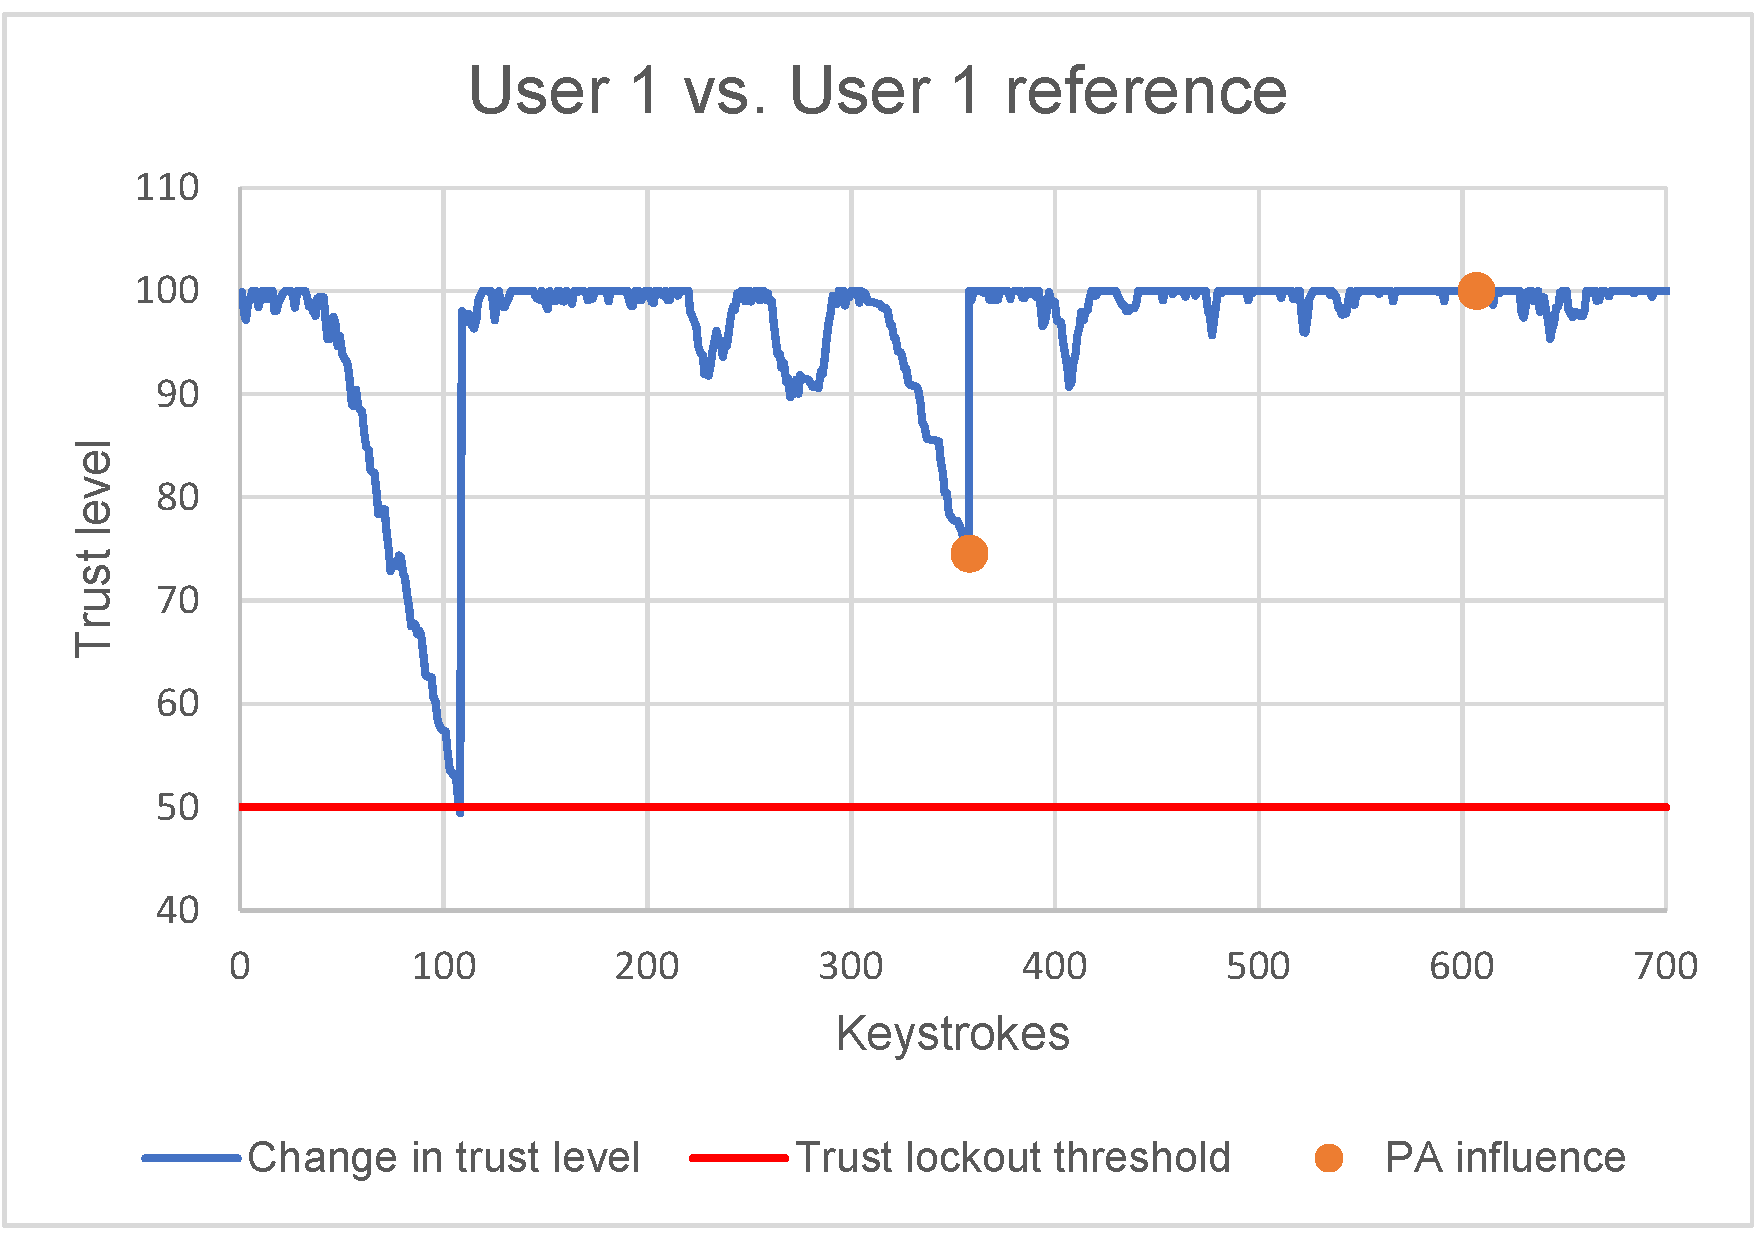
\includegraphics[width=0.8\textwidth]{figures/decision-lvl-genuine-250BL.pdf}
%    \caption{Decision level fusion with User 1 as genuine user. $\text{Up} = 100.1\%, \text{Down} = 60\%$. $BL = 250$.}
%    \label{fig:decision-lvl-genuine-250BL}
%\end{figure}
%
%\begin{figure}[ht]
%    \centering
%    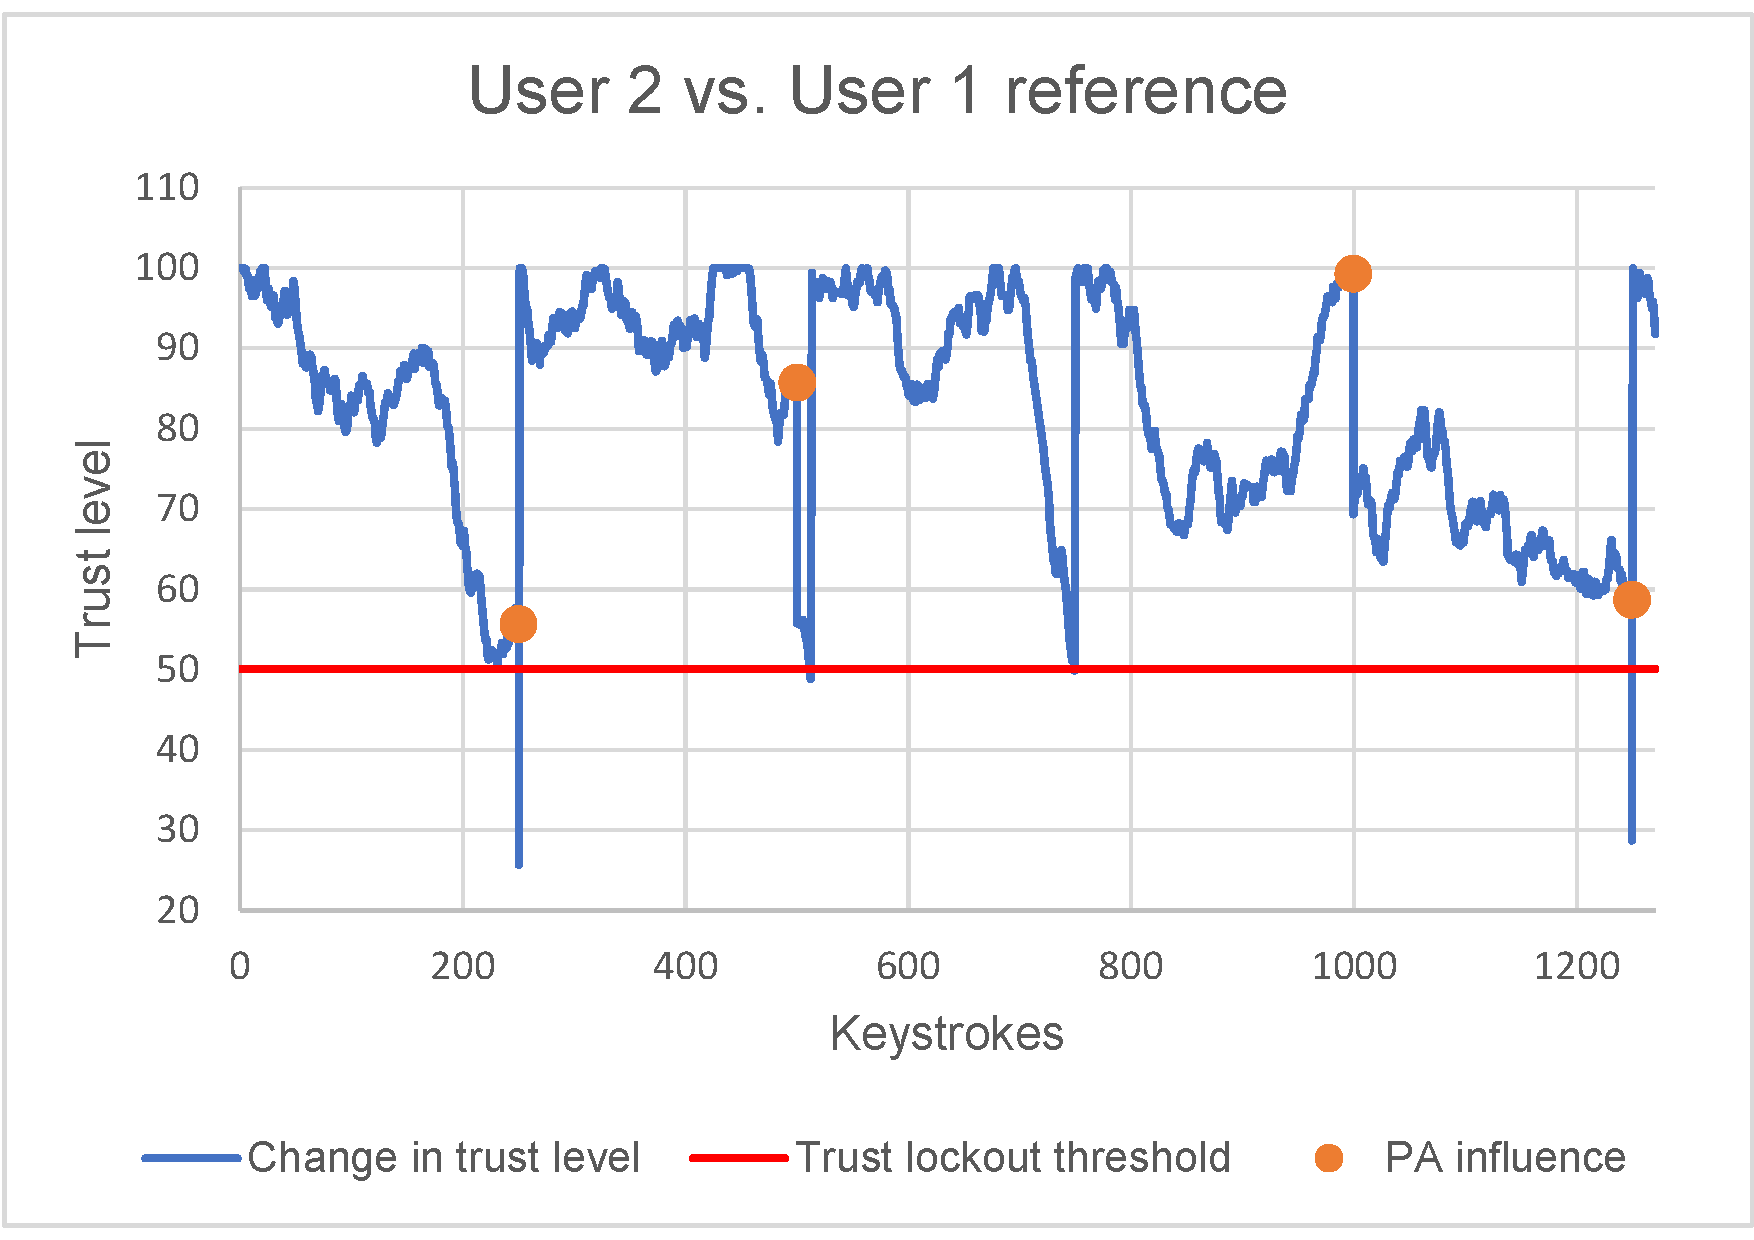
\includegraphics[width=0.8\textwidth]{figures/decision-lvl-user2-vs-user1-250BL.pdf}
%    \caption{Decision level fusion with User 2 as imposter. $\text{Up} = 100.1\%, \text{Down} = 60\%$. $BL = 250$.}
%    \label{fig:decision-lvl-user2-vs-user1-BL100}
%\end{figure}

\section{Score level fusion}
\label{sec:analysis-score-lvl}
As with the decision level fusion, the score level fusion is also based on $T_{\text{range}}$.
During testing, we gave the DTM's sigmoid function for PA influence, $\textit{Sig}_{\text{PA}}$, a height that allowed a change of trust between 0 and 50.001.
\Cref{fig:trustProgressScoreLevel} shows how the score level fusion allows the PA influence to have varying degrees of impact depending on the dissimilarity scores calculated from probe blocks.
The first of the three times the PA system kicked in, it caused a lockout by lowering the trust by 39 levels.
It kicked in again at keystroke number 333, lowering the trust by 35, meaning that block was slightly more similar to the reference than the first.
While it did not cause a direct lockout, it assisted the CA system enough for it to lock the user out at at keystroke number 535.
Lastly, we see the PA system being less decisive in its dissimilarity score, causing a drop of only 7 levels.
Because the trust level was already close to $T_{\text{lockout}}$, it still managed to nudge the trust level down just enough to cause a lockout slightly before the CA subsystem would have done so itself.

\begin{figure}[ht]
    \centering
    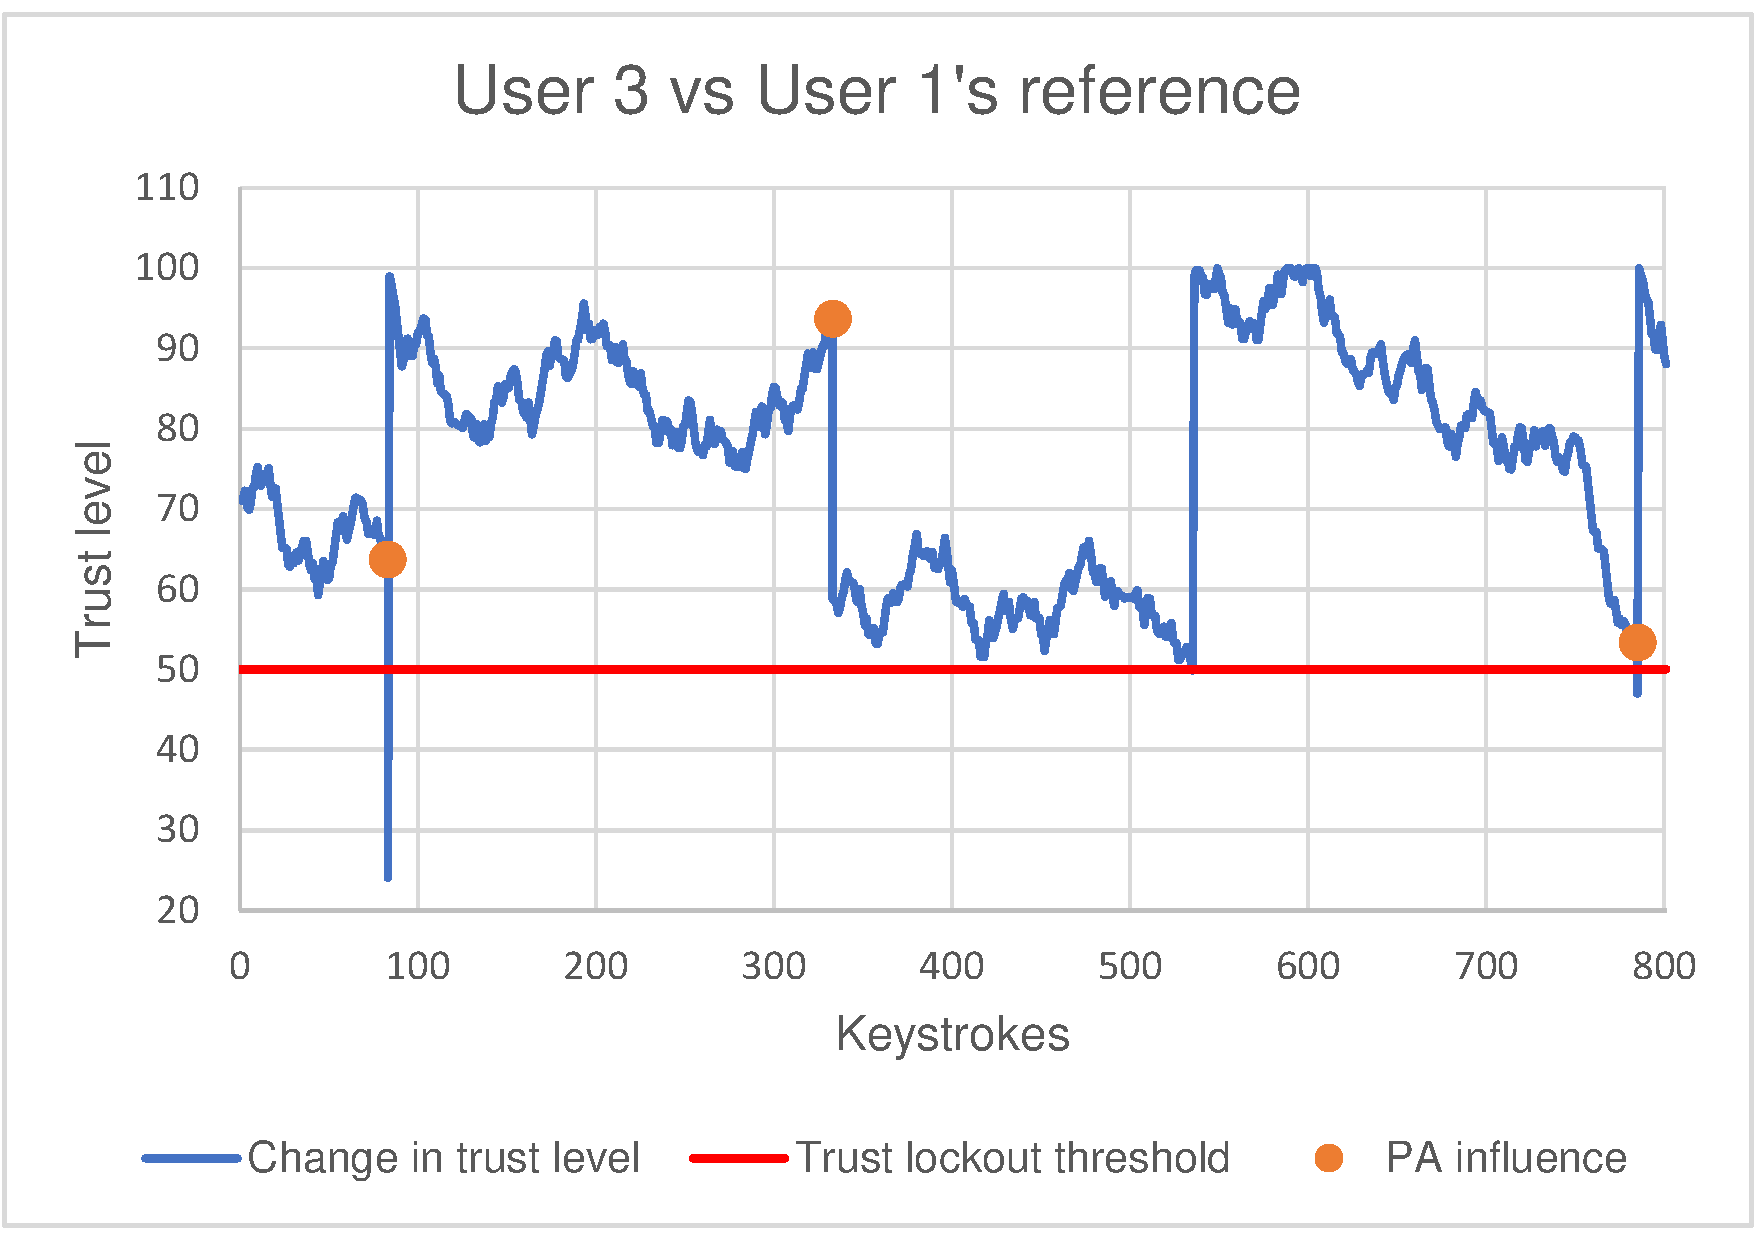
\includegraphics[width=0.8\textwidth]{figures/trustProgressScoreLevel.pdf}
    \caption{Example of score level fusion with $\text{block size} = 250$, where User 3 was tested as an imposter vs User 1's reference. DTM parameters for $\textit{Sig}_{\text{PA}}$ were as follows: $A = \text{personal} + 0.5 \text{ tolerance}$, $B = 0.1$, $C = 50.001$.}
    \label{fig:trustProgressScoreLevel}
\end{figure}

\subsection{Results}
\label{sec:analysis-score-lvl-results}
The performance was tested by adjusting the width of $\textit{Sig}_{\text{PA}}$, as well as the PA tolerance.
The tolerance was added to the user's mean score from the validation set, similarly to the decision level fusion, however in this case it controlled the threshold for reward and penalty.
Increasing the tolerance essentially shifted $\textit{Sig}_{\text{PA}}$ towards the right.
Following are the results achieved by adjusting these parameters for different block sizes.

\subsubsection{Block size 500}
We were able to find settings improving the ANIA rating of the original CA system also with this fusion scheme. %albeit less successfully than with decision level fusion.
\Cref{tab:analysis-score-level-BL500} shows the performance using different $\textit{Sig}_{\textit{PA}}$ widths with blocks size 500.
There are more results available \Cref{sec:app-score-BL500}, however \Cref{tab:analysis-score-level-BL500} is focused on results where either the ANGA or ANIA is comparable to the original CA system.
%\todo{Refer directly to attachments.}
Similarly to decision level fusion, the ANGA was boosted to around 8500 when the ANIA was around the same as the CA system, being 623.
The best widths for boosting the ANGA seemed to be 0.25 and 0.3 for our specific combination and dataset, giving 8520 and 8540 ANGA while having a lower ANIA than the CA system, as well as one less undetected imposter.



\begin{table}[htbp]
\centering
\begin{tabular}{llrrr}
\hline
\textbf{Width}        & \textbf{Tolerance} & \textbf{ANGA} & \textbf{ANIA} & \textbf{\#Imp. ND} \\ \hline
\multirow{2}{*}{0.05} & 0.55               & 8097          & 539           & 13(0.6\%)          \\
                      & 0.7                & 8550          & 631           & 18(0.9\%)          \\ \hline
\multirow{2}{*}{0.1}  & 0.5                & 8094          & 560           & 13(0.6\%)          \\
                      & 0.6                & 8497          & 611           & 15(0.7\%)          \\ \hline
\multirow{2}{*}{0.25} & 0.3                & 7892          & 527           & 11(0.5\%)          \\
                      & 0.5                & 8540          & 614           & 17(0.8\%)          \\ \hline
\multirow{2}{*}{0.3}  & 0.262               & 8158          & 533          & 11(0.5\%)          \\
                      & 0.5                & 8520          & 613           & 17(0.8\%)          \\ \hline
\multirow{2}{*}{0.45} & 0.2                & 7914          & 552           & 14(0.7\%)          \\
                      & 0.5                & 8500          & 621           & 18(0.9\%)          \\ \hline
\multirow{2}{*}{0.65} & 0.3                & 8085          & 587           & 16(0.8\%)          \\
                      & 0.5                & 8432          & 629           & 18(0.9\%)          \\ \hline
\end{tabular}
\caption{Selected portions of score level fusion results with block size 500, sorted by the width of $\textit{Sig}_{\text{PA}}$.}
\label{tab:analysis-score-level-BL500}
\end{table}

Width 0.3 also seems to be the best performer for decreasing ANIA, as it was lowered to 533 while having a higher ANGA than the CA system's 8087.
The number of undetected imposters was also seven less.
In order to be able to compare the result to the decision level fusion with block size 500, we attempted to lower the tolerance in hopes of bringing the ANGA down to a rating closer to 8087.
This resulted in a 7943 ANGA and 530 ANIA, which was worse than the decision level fusion.

%This fusion scheme was also able to improve the ANIA rating of the original CA system, albeit less so than decision level fusion.


\subsubsection{Block size 250}
We observed that a larger width for $\textit{Sig}_{\text{PA}}$ was needed with block size 250.
This was clear, as widths 0.05 and 0.3 decreased the original CA system's performance apart from having one less undetected imposter, as seen in \Cref{tab:analysis-score-level-BL250}.
Both of these widths had lower ANGAs and higher ANIAs, meaning genuine users were locked out faster, while imposters had larger windows of opportunity.
At larger widths, we saw more reasonable results.
A possible cause could be the fact that smaller block sizes result in less accurate PA comparisons, as was shown in \Cref{fig:block-lengths-ROC}.
With larger sigmoid widths, comparison scores will on average cause smaller changes to the trust level. 
In other words, comparison scores are given more "wiggle room" before the influence on the trust level becomes very large, which prevents inaccurate scores to cause too much damage.
While less accurate, the smaller block sizes also cause PA comparison scores to be produced more rapidly.
Therefore, reducing the impact that each of these scores have on the trust level by increasing the width seems logical, and we believe this to be a likely explanation.

\begin{table}[htbp]
\centering
\begin{tabular}{llrrr}
\hline
\textbf{Width}        & \textbf{Tolerance} & \textbf{ANGA} & \textbf{ANIA} & \textbf{\#Imp. ND} \\ \hline
0.05                 & 0.7                & 8047          & 652           & 17(0.8\%)          \\ \hline
0.3                  & 0.7                & 7912          & 629           & 17(0.8\%)          \\ \hline
\multirow{2}{*}{0.5} & 0.35               & 7906          & 572           & 15(0.7\%)          \\
                     & 0.45               & 8745          & 623           & 21(1\%)            \\ \hline
\multirow{2}{*}{0.7} & 0.2                & 7946          & 538           & 14(0.7\%)          \\
                     & 0.5                & 8705          & 640           & 22(1.1\%)          \\ \hline
\end{tabular}
\caption{Selected excepts of score level fusion results with block size 250, sorted by the width of $\textit{Sig}_{\text{PA}}$.}
\label{tab:analysis-score-level-BL250}
\end{table}

\Cref{tab:analysis-score-level-BL250} shows that the best result for decreasing ANIA using this block size was achieved with $\text{width} = \text{0.7}$, and $\text{tolerance} = \text{0.2}$.
It gave an ANGA of 7946 and ANIA of 538, which was not as effective as the best ANIA decreasing result with block size 500.
%However, the ANIA was higher than what was achieved with block size 500, and the ANGA was also lower.
On the other hand, we saw positive results for increasing ANGA using block size 250.
With $\text{width} = \text{0.5}$, and $\text{tolerance} = \text{0.45}$, it gave an ANGA of 8745 while having the same ANIA as the original system.
This was the best ANGA improvement observed in the project's analysis phase, being an 8.14\% increase.

Just as with decision level fusion, we see that smaller block sizes are better at improving ANGA, while larger block sizes are better at decreasing ANIA.
Before the analysis, we expected otherwise.
Specifically, we expected large block sizes to be better for reducing ANIA and shorter block lengths to be better for increasing ANGA.
Because the CA subsystem has the ability to rapidly drop imposters' trust levels and locking them out after a small amount of keystrokes. 
Therefore, we expected large block sizes to cause the PA subsystem to kick in too seldom to significantly increase imposter detection rates, since blocks are reset every time the CA subsystem causes a lockout on its own.
More research is needed to conclude on why larger block sizes seem better for lowering ANIA ratings.


%best impact on the overall performance, since blocks are reset after every lockout.



%Seeing this in both fusion schemes is probably no coincidence, and it raises the question of what causes such behavior.
%Looking back at \Cref{tab:PA-block-lengths}, we can see that for smaller block sizes, the tolerance levels need to be significantly higher in order to achieve high ANGA ratings.
%A possible reason is that the PA settings we have used have had lower FNMR than FMR in order to achieve reasonably high ANGA ratings.
%Therefore, when smaller block sizes are used, the PA system kicks in more often, and therefore makes



\subsubsection{Block size 100}
We performed limited testing of block size 100 with score level fusion.
However, we did test a number of different sigmoid widths, and the results in \Cref{tab:analysis-score-level-BL100} show that for ANGA values close to that of the CA system, it showed worse ANIA ratings for all widths.
We were unable to find a setting with this block size which improved the CA system's performance.
It is possible that increasing the width of $\textit{Sig}_{\text{PA}}$ is not enough to reduce the impact of inaccurate comparisons.
This issue could be interesting to investigate further.
Reducing the \text{height} of the sigmoid function to forcibly restrict the PA system from causing too large changes to the trust level could yield different results.
%It is possible that due to inaccurate comparisons, the \text{height} of the sigmoid needs to be reduced, forcibly restricting the PA system from causing too large changes to the trust level.
%More research is needed to investigate this issue.

\begin{table}[htbp]
\centering
\begin{tabular}{llrrr}
\hline
\textbf{Width} & \textbf{Tolerance} & \textbf{ANGA} & \textbf{ANIA} & \textbf{\#Imp. ND} \\ \hline
0.05           & 0.8                & 8043          & 935           & 35(1.7\%)          \\ %\hline
0.15           & 0.6                & 8010          & 771           & 30(1.4\%)          \\ %\hline
0.25           & 0.4                & 6990          & 576           & 22(1.1\%)          \\ %\hline
0.3            & 0.5                & 7927          & 715           & 29(1.4\%)          \\ %\hline
0.5            & 0.4                & 7866          & 649           & 25(1.2\%)          \\ %\hline
0.7            & 0.4                & 8015          & 652           & 23(1.1\%)          \\ %\hline
0.9            & 0.4                & 8063          & 656           & 21(1\%)            \\ %\hline
1.2            & 0.4                & 7981          & 656           & 22(1.1\%)          \\ %\hline
\end{tabular}
\caption{Selected excepts of score level fusion results with block size 100, sorted by the width of $\textit{Sig}_{\text{PA}}$.}
\label{tab:analysis-score-level-BL100}
\end{table}
%With smaller block size, more width is needed.

\section{Overview of the best results}
\label{sec:analysis-overview-best-results}
We conclude the analysis of detection performance by presenting an overview the best results for increasing ANGA and decreasing ANIA, both of which have been discussed in \Cref{sec:analysis-decision-lvl-results,sec:analysis-score-lvl-results}.
Here, we can see how the users fell into different categories before and after combining the systems.
\Cref{tab:CA-detailed-performance} shows the detailed results of the original CA system.
When comparing it to the best result for increasing ANGA, in the upper half of \Cref{tab:best-results}, we see that the distribution of users in different categories is very similar.
One user was moved from -/+ to +/+, which was a small but positive change.
This means that the combined system cause one more user to never be locked out.
While the total number of imposters not detected went up by 0.1\%, the genuine user was on average able to type 658 characters more, an increase of 8.14\%.

In the lower half of \Cref{tab:best-results}, we see that the best result for decreasing ANIA showed some more changes on user categories.
This setting also had one more user in the best category compared to the CA system.
There were also six less users who had at least one undetected imposter, as seen in the decreases of users in the +/- and -/- categories.
The total number of imposters who were not detected was therefore decreased, down by 7.
This, in addition to imposters on average being able to type $\text{623}-\text{508} = 115$ less characters before being locked out, was overall a positive result.

\begin{table}[ht]
\centering
\begin{tabular}{lrrrr}
\hline
\textit{} Category & \#Users & ANGA & ANIA & \#Imp. ND \\ \hline
+/+ & 6  & 17409 & 269  & 0  \\
+/- & 1  & 12256 & 485  & 1  \\
-/+ & 30 & 6682  & 390  & 0  \\
-/- & 9  & 6091  & 1650 & 17 \\ \hline
Summary & 46 & 8087  & 623  & 18(0.9\%) \\ \hline
\end{tabular}
\caption{Detailed performance results of the CA configuration used in the combined system.}
\label{tab:CA-detailed-performance}
\end{table}

\begin{table}[h]
\centering
\begin{tabular}{llrrrr}
\hline
\textit{} & Category & \#Users & ANGA & ANIA & \#Imp. ND \\ \hline
\multirow{4}{*}{\textit{\begin{tabular}[c]{@{}l@{}}Score level\\ Block size 250\end{tabular}}} & +/+ & 7 & 21735 & 336 &  \\
 & +/- & 1 & 12256 & 483 & 1 \\
 & -/+ & 29 & 6130 & 328 &  \\
 & -/- & 9 & 6678 & 1815 & 20 \\ \cline{2-6} 
\textit{} & Summary & 46 & 8745 & 623 & 21(1\%) \\ \hline
\multirow{4}{*}{\textit{\begin{tabular}[c]{@{}l@{}}Decision level\\ Block size 500\end{tabular}}} & +/+ & 7 & 21979 & 308 &  \\
 & +/- & 0 &  &  &  \\
 & -/+ & 35 & 5328 & 353 &  \\
 & -/- & 4 & 7945 & 2214 & 11 \\ \cline{2-6} 
\textit{} & Summary & 46 & 8089 & 508 & 11(0.5\%) \\ \hline
\end{tabular}
\caption{CA results achieved by adjusting Single Occurrence (SO) and No Occurrences (NO) parameters. DTM parameters were $A = 1.85$, $B = 0.28$, $C = 1$ and $T_{\text{lockout}} = 90$.}
\label{tab:best-results}
\end{table}

\section{Computational impact}
\label{sec:analysis-computational-impact}
Regarding \textit{research sub-question 1}, we realize that computation speeds are highly dependent on a number of factors such as processing power, programming language, choice of classifier and number of considered features.
Still, we can mention that our CA system performs a comparison of a single keystroke in 0.2 milliseconds on average.
For our PA system, the average computing time for processing blocks of 500, 250 and 100 keystrokes was 75.2, 46 and 25.7 milliseconds, respectively.
These times were collected by finding the user with the largest reference in terms of unique mono- and digraphs, and running their validation set against their own reference.
The systems were developed in MATLAB 2017, and were run on an Intel Core i7, on a single thread at 2.4 GHz frequency.
While the speeds were reasonable, they could be further improved by for example using more a low-level programming language, not to mention multi-threading.

What is most interesting to discuss is the computational impact of combining the systems.
The most important factor here is the PA subsystem's block size.
In an example where the combined system has to process 100,000 keystrokes and the block size is 100, a crude way to calculate the number of times the PA system could kick in is simply $100,000/100 = 1000$, which is the maximum.
For block size 250 and 500, it could kick in at most 400 and 200 times, respectively.
However, what must also be considered is the fact that the likelihood of the CA subsystem locking out the user before a block is filled up increases with larger block sizes.
When that happens, the PA subsystem resets and waits until enough keystrokes are recorded to fill a new block.
This further reduces computational costs when using large block sizes.

It is also important to discuss the difference between the tests we have performed and a real-time system.
During testing, we ran both the CA and PA subsystems on the same thread.
This was to avoid having the CA subsystem continuing to adjust the trust level while the PA subsystem was still processing a block probe.
If that were to happen, our results could have been less accurate.
An example could be the CA subsystem increasing an imposter's trust level before the PA subsystem had finished processing a block, and that increase of trust preventing the PA subsystem's influence from locking the user out.
Situations like these could therefore alter the performance readings.
This would not matter in a deployed real-time system as the objective would simply be to lock out imposters, and not to measure performance.
Therefore, the PA subsystem could process a block parallel to the CA system processing keystrokes with multithreading, further reducing computational impact.



